% ------------------------------------------------------------------------
% ------------------------------------------------------------------------
% Monografia Peacon
% Trabalho de Conclusão de Curso
% Baseia-se no documento modelo de TCC do abntex2
% Para saber mais, acesse https://github.com/abntex/abntex2
% ------------------------------------------------------------------------
% ------------------------------------------------------------------------

\documentclass[
		% -- opções da classe memoir --
		12pt,				% tamanho da fonte
		openright,			% capítulos começam em pág ímpar (insere página vazia caso preciso)
		oneside,			% para impressão em verso e anverso. Oposto a oneside
		a4paper,			% tamanho do papel. 
		% -- opções da classe abntex2 --
		chapter=TITLE,		% títulos de capítulos convertidos em letras maiúsculas
		%section=TITLE,		% títulos de seções convertidos em letras maiúsculas
		%subsection=TITLE,	% títulos de subseções convertidos em letras maiúsculas
		%subsubsection=TITLE,% títulos de subsubseções convertidos em letras maiúsculas
		% -- opções do pacote babel --
		english,			% idioma adicional para hifenização
		brazil				% o último idioma é o principal do documento
	]{abntex2}


% ----------------------------------------------------------
% Pacotes básicos 
% ----------------------------------------------------------
%\usepackage{helvet}			
\usepackage[scaled]{helvet}
\renewcommand*\familydefault{\sfdefault} 	% Only if the base font of the document is to be sans serif
										% Foi necessário para acertar o documento, continha diversos erros
\usepackage[T1]{fontenc}		% Selecao de codigos de fonte.
\usepackage[utf8]{inputenc}	% Codificacao do documento (conversão automática dos acentos)
\usepackage{lastpage}		% Usado pela Ficha catalográfica
\usepackage{indentfirst}		% Indenta o primeiro parágrafo de cada seção.
\usepackage{color}			% Controle das cores
\usepackage{graphicx}		% Inclusão de gráficos
\usepackage{microtype} 		% para melhorias de justificação
% ----------------------------------------------------------
		

% ----------------------------------------------------------
% Pacotes adicionais, usados apenas no âmbito do Modelo Canônico do abnteX2
%% ----------------------------------------------------------
\usepackage{lipsum}				% para geração de dummy text
\usepackage{customizacoes} 		% customizações feitas pelo autor
% ----------------------------------------------------------


% ----------------------------------------------------------
% Pacotes de citações
% ----------------------------------------------------------
\usepackage[alf]{abntex2cite}				% Citações padrão ABNT

% ----------------------------------------------------------
% CONFIGURAÇÕES DE PACOTES
% ----------------------------------------------------------

% ----------------------------------------------------------
% Configurações do pacote backref
% ----------------------------------------------------------
\definecolor{thered}{rgb}{0.65,0.04,0.07}
\definecolor{thegreen}{rgb}{0.06,0.44,0.08}
\definecolor{thegrey}{gray}{0.5}
\definecolor{theshade}{rgb}{1,1,0.97}
\definecolor{theframe}{gray}{0.6}
% ----------------------------------------------------------



% ----------------------------------------------------------
% Informações de dados para CAPA e FOLHA DE ROSTO
% ----------------------------------------------------------

\titulo{Aplicação de Redes Neurais Artificiais no Balanceamento de Carga em Serviços de Nuvem}
\autor{Karoline Kimiko Figueiredo Setoue}
\local{Bauru}
\data{2017}
\orientador{Prof. Dr. Kelton Augusto Pontara da Costa}
%\coorientador{Prof. Dr. João Paulo Papa}
\instituicao{%
  Universidade Estadual Paulista "Júlio de Mesquita Filho"
  \par
  Faculdade de Ciências - Campus Bauru
  \par
  Departamento de Computação
}
\tipotrabalho{Monografia (Trabalho de Conclusão de Curso)}
% O preambulo deve conter o tipo do trabalho, o objetivo, 
% o nome da instituição e a área de concentração 
% foi necessário utilizar \~{a} e etc para os acentos por problemas na geração do PDF
\preambulo{Trabalho de Conclus\~{a}o do Curso de Bacharelado em Ciência da Computação apresentado ao Departamento de Computa\c{c}\~{a}o da Faculdade de Ci\^{e}ncias da Universidade Estadual Paulista ``J\'{ú}lio de Mesquita Filho'' – UNESP, C\^{a}mpus de Bauru.}

% ----------------------------------------------------------


% ----------------------------------------------------------
% Configurações de aparência do PDF final
% ----------------------------------------------------------

% alterando o aspecto da cor azul
\definecolor{blue}{RGB}{0,0,0}

% informações do PDF
\makeatletter
\hypersetup{
     	%pagebackref=true,
		pdftitle={\@title}, 
		pdfauthor={\@author},
    	pdfsubject={\imprimirpreambulo},
	    pdfcreator={LaTeX with abnTeX2},
		pdfkeywords={beacon}{raspberry pi}{internet das coisas}{abntex2}{trabalho acadêmico}, 
		colorlinks=true,       		% false: boxed links; true: colored links
    	linkcolor=blue,          	% color of internal links
    	citecolor=blue,        		% color of links to bibliography
    	filecolor=magenta,      		% color of file links
		urlcolor=blue,
		bookmarksdepth=4
}
\makeatother
% ----------------------------------------------------------


% ----------------------------------------------------------
% Espaçamentos entre linhas e parágrafos 
% ----------------------------------------------------------

% O tamanho do parágrafo é dado por:
\setlength{\parindent}{1.3cm}

% Controle do espaçamento entre um parágrafo e outro:
\setlength{\parskip}{0.2cm}  % tente também \onelineskip

% ----------------------------------------------------------
% compila o indice
% ----------------------------------------------------------
\makeindex
% ----------------------------------------------------------


% ----------------------------------------------------------
% Configurações de projeto
% ----------------------------------------------------------
\newif\iffinal
\finaltrue % define se é um arquivo final, se for não for retira umas partes. 

\newif\ifrelatorio
\relatoriofalse % define se é um arquivo final, se for não for retira umas partes. 

\newif\ifabstract
\abstractfalse % define se mostra o abstract em inglês ou não.

\newif\ifresumo
\resumotrue % define se mostra o resumo ou não.

\newif\ifficha
\fichafalse % define se mostra a ficha catalográfica ou não
% ----------------------------------------------------------


% ----------------------------------------------------------
% Início do documento
% ----------------------------------------------------------
\begin{document}

% Seleciona o idioma do documento (conforme pacotes do babel)
%\selectlanguage{english}
\selectlanguage{brazil}

% Retira espaço extra obsoleto entre as frases.
\frenchspacing 

% ----------------------------------------------------------
% ELEMENTOS PRÉ-TEXTUAIS
% ----------------------------------------------------------
\pretextual


% ----------------------------------------------------------
% Capa
% ----------------------------------------------------------
\imprimircapa
% ----------------------------------------------------------


% ----------------------------------------------------------
% Folha de rosto
% (o * indica que haverá a ficha bibliográfica)
% ----------------------------------------------------------
\imprimirfolhaderosto
% ----------------------------------------------------------


% ----------------------------------------------------------
% Inserir a ficha catalográfica
% ----------------------------------------------------------

% Isto é um exemplo de Ficha Catalográfica, ou "Dados internacionais de
% catalogação-na-publicação''. Você pode utilizar este modelo como referência. 
% Porém, provavelmente a biblioteca da sua universidade lhe fornecerá um PDF
% com a ficha catalográfica definitiva após a defesa do trabalho. Quando estiver
% com o documento, salve-o como PDF no diretório do seu projeto e substitua todo
% o conteúdo de implementação deste arquivo pelo comando abaixo:
%
% \begin{fichacatalografica}
%     \includepdf{fig_ficha_catalografica.pdf}
% \end{fichacatalografica}

%\begin{fichacatalografica}
%	\sffamily
%	\vspace*{\fill}					% Posição vertical
%	\begin{center}					% Minipage Centralizado
%		\fbox{\begin{minipage}[c][8cm]{13.5cm}		% Largura
%				\small
%				\imprimirautor
%				%Sobrenome, Nome do autor
%				
%				\hspace{0.5cm} \imprimirtitulo / \imprimirautor. --
%				\imprimirlocal, \imprimirdata-
%				
%				\hspace{0.5cm} \pageref{LastPage} p. : il. (algumas color.) ; 30 cm.\\
%				
%				\hspace{0.5cm} \imprimirorientadorRotulo~\imprimirorientador\\
%				
%				\hspace{0.5cm}
%				\parbox[t]{\textwidth}{\imprimirtipotrabalho~--~\\ \imprimirinstituicao,
%					\imprimirdata.}\\
%				
%				\hspace{0.5cm}
%				1. Balanceamento de Cargas.
%				2. Redes Neurais Artificiais.
%				3. Computação em Nuvem.
%				I. \imprimirorientador.
%				II. Universidade Estadual Paulista "Júlio de Mesquita Filho".
%				III. Faculdade de Ciências.
%				IV. \imprimirtitulo
%			\end{minipage}}
%		\end{center}
%	\end{fichacatalografica}

\begin{fichacatalografica}
	\ttfamily
	\vspace*{\fill}					% Posição vertical
	\hspace{1.5cm}
	\begin{centering}	% Minipage Centralizado
		\fbox{\begin{minipage}[c][7.5cm]{12.5cm}		% Largura
				\footnotesize
				\vspace{0.3cm}
				\hspace{2.0cm} Setoue, Karoline Kimiko Figueiredo.
				%Sobrenome, Nome do autor
				
				\hspace{2.0cm} \parbox[t]{\textwidth}{\hspace{0.5cm} Aplicação de redes neurais artificiais no balanceamento de carga em serviços de nuvem / \imprimirautor, \imprimirdata} \\	
				
				\hspace{2.0cm} \parbox[t]{\textwidth}{\hspace{0.5cm} \pageref{LastPage} f. : il.} \\
				
				\hspace{2.0cm} \parbox[t]{\textwidth}{\hspace{0.5cm} \imprimirorientador} \\
				
				\hspace{2.0cm} \parbox[t]{\textwidth}{\hspace{0.5cm} Monografia (Graduação)~--~Universidade Estadual \\ Paulista. Faculdade de Ciências, Bauru, 2017 \\}  
				\\	
				
				
				\hspace{2.0cm} \parbox[t]{\textwidth}{\hspace{0.5cm} 1. Balanceamento de carga. 2. Redes neurais artificiais. \\ 3. Computação em nuvem. I. Universidade \\ Estadual Paulista. Faculdade de Ciências. II. Título.}	
			\end{minipage}}
		\end{centering}
\end{fichacatalografica}
% ----------------------------------------------------------


% ----------------------------------------------------------
% Inserir errata
% ----------------------------------------------------------
%\begin{errata}
%Elemento opcional da \citeonline[4.2.1.2]{NBR14724:2011}. Exemplo:

%\vspace{\onelineskip}

%FERRIGNO, C. R. A. \textbf{Tratamento de neoplasias ósseas apendiculares com
%reimplantação de enxerto ósseo autólogo autoclavado associado ao plasma
%rico em plaquetas}: estudo crítico na cirurgia de preservação de membro em
%cães. 2011. 128 f. Tese (Livre-Docência) - Faculdade de Medicina Veterinária e
%Zootecnia, Universidade de São Paulo, São Paulo, 2011.

%\begin{table}[htb]
%\center
%\footnotesize
%\begin{tabular}{|p{1.4cm}|p{1cm}|p{3cm}|p{3cm}|}
%  \hline
%   \textbf{Folha} & \textbf{Linha}  & \textbf{Onde se lê}  & \textbf{Leia-se}  \\
%    \hline
%    1 & 10 & auto-conclavo & autoconclavo\\
%   \hline
%\end{tabular}
%\end{table}

%\end{errata}
% ----------------------------------------------------------


% ----------------------------------------------------------
% Inserir folha de aprovação
% ----------------------------------------------------------

% Isto é um exemplo de Folha de aprovação, elemento obrigatório da NBR
% 14724/2011 (seção 4.2.1.3). Você pode utilizar este modelo até a aprovação
% do trabalho. Após isso, substitua todo o conteúdo deste arquivo por uma
% imagem da página assinada pela banca com o comando abaixo:
%
% \includepdf{folhadeaprovacao_final.pdf}
%
\begin{folhadeaprovacao}
	
	\begin{center}
		{\ABNTEXchapterfont\large\imprimirautor}
		
		\vspace*{\fill}\vspace*{\fill}
		\begin{center}
			\ABNTEXchapterfont\bfseries\Large\imprimirtitulo
		\end{center}
		\vspace*{\fill}
		
		\hspace{.45\textwidth}
		\begin{minipage}{.5\textwidth}
			\imprimirpreambulo
		\end{minipage}%
		\vspace*{\fill}
	\end{center}
	
	\center Banca Examinadora
	\begin{center}
		\vspace*{0.5cm}
		\textbf{\imprimirorientador} \\ Orientador \\ Universidade Estadual Paulista "Júlio de Mesquita Filho" \\ Departamento de computação\\ Faculdade de Ciências \\
	\end{center}
	\begin{center}
		\vspace*{0.5cm}
		\textbf{Profa. Dra. Simone das Graças Domingues Prado} \\ Universidade Estadual Paulista "Júlio de Mesquita Filho" \\ Departamento de computação\\ Faculdade de Ciências \\
	\end{center}
	\begin{center}
		\vspace*{0.5cm}
		\textbf{Profa. Dra. Roberta Spolon} \\ Universidade Estadual Paulista "Júlio de Mesquita Filho" \\ Departamento de computação\\ Faculdade de Ciências \\
	\end{center}
	%\assinatura{\textbf{Professor} \\ Convidado 3}
	%\assinatura{\textbf{Professor} \\ Convidado 4}
	
	\begin{center}
		\vspace*{0.5cm}
		\par
		{Bauru, 07 de Fevereiro de 2017.}
		\vspace*{1cm}
	\end{center}
	
\end{folhadeaprovacao}
% ----------------------------------------------------------


% ----------------------------------------------------------
% Dedicatória
% ----------------------------------------------------------
\ifrelatorio
	\begin{dedicatoria} 
		\vspace*{\fill}
		\centering
		\noindent
		\textit{ Este trabalho é dedicado às crianças adultas que,\\
				quando pequenas, sonharam em se tornar cientistas.} 
		\vspace*{\fill}
	\end{dedicatoria}
\fi
% ----------------------------------------------------------


% ----------------------------------------------------------
% Agradecimentos
% ----------------------------------------------------------
\iffinal
	\begin{agradecimentos}
	
	Agradeço a todos os familiares por todo o incentivo e apoio. Especialmente às minhas irmãs, por estarem ao meu lado ao longo desta jornada. 
	
	Aos meus amigos, por todo apoio, incentivo, companheirismo e por me mostrarem que não 
	é preciso estar perto para estar presente. Sou grata por todos os momentos que compartilhamos. 
	
	Aos meus professores da Unesp, por todo o conhecimento compartilhado, especialmente ao Prof. Dr. Kelton, pela orientação ao longo deste projeto. 	
	
	Ao LTIA e ao Prof. Dr. Eduardo Morgado por me proporcionar oportunidades tão boas em um ambiente com tantas pessoas excepcionais que levarei comigo ao longo da vida. 
	
	
	
	
	
	
	


	\end{agradecimentos}
\fi
% ----------------------------------------------------------


% ----------------------------------------------------------
% Epígrafe
% ----------------------------------------------------------
\iffinal
	\begin{epigrafe}
		\vspace*{\fill}
			\begin{flushright}
			
				
		\textit{"Mundo mundo vasto mundo..."\\
			(Carlos Drummond de Andrade)}
		\textit{""\\
				}
		\end{flushright}
	\end{epigrafe}
\fi
% ----------------------------------------------------------


% ----------------------------------------------------------
% RESUMOS
% ----------------------------------------------------------
\ifresumo
	% resumo em português
	\setlength{\absparsep}{18pt} % ajusta o espaçamento dos parágrafos do resumo
	\begin{resumo}

		O conceito de computação em nuvem tem se tornado popular nos últimos anos. Seu objetivo é prover serviços de acesso à aplicações e arquivos por meio da internet de maneira flexível e simples. Neste contexto, explorar maneiras de garantir este acesso de maneira eficiente torna-se uma tarefa importante na área de computação. Tendo isto em vista, o presente trabalho apresenta um protótipo de aplicação de balanceamento de cargas em uma arquitetura de computação em nuvem utilizando Redes Neurais Artificiais como técnica para distribuição das cargas de requisições. A construção da aplicação consiste na incorporação da rede neural no monitoramento e ajuste dos pesos em cada servidor do sistema em nuvem para os quais as requisições serão direcionadas. 
		
		\textbf{Palavras-chave}: Redes Neurais Artificiais. Computação em Nuvem. Balanceamento de Carga.
 			
	\end{resumo}
	
	% resumo em inglês
	\begin{resumo}[Abstract]
	 	\begin{otherlanguage*}{english}
			
		The concept of cloud computing has become popular in recent years. Its goal is to provide services that allows access to applications and files through the Internet in a flexible and simple way. In this context, exploring ways to secure this access efficiently becomes an important task in Computer Science. Therefore, the present work presents a load balancing application prototype in a cloud computing architecture using Artificial Neural Networks as a technique for load distribution of requests. The application consists in a neural network applied to monitoring and adjustment of the weights for each server to which requests are directed.
			 
		\textbf{Keywords}: Artificial Neural Networks. Cloud Computing. Load Balancing.
		\end{otherlanguage*}
	\end{resumo}
	
\fi
% ----------------------------------------------------------


% ----------------------------------------------------------
% inserir lista de ilustrações
% ----------------------------------------------------------
\iffinal
	\pdfbookmark[0]{\listfigurename}{lof}
	\listoffigures*
	\cleardoublepage
\fi
% ----------------------------------------------------------


% ----------------------------------------------------------
% inserir lista de tabelas
% ----------------------------------------------------------
\iffinal
	\pdfbookmark[0]{\listtablename}{lot}
	\listoftables*
	\cleardoublepage
\fi
% ----------------------------------------------------------


% ----------------------------------------------------------
% inserir lista de abreviaturas e siglas
% ----------------------------------------------------------
\iffinal
	\begin{siglas}
			\item[ANN] \textit{Artificial Neural Networks}    
			\item[AWS] \textit{Amazon Web Services}    
			\item[RNA] \textit{Rede Neural Artificial}    
	\end{siglas}
\fi
% ----------------------------------------------------------


% ----------------------------------------------------------
% inserir lista de símbolos
% ----------------------------------------------------------
%\iffinal
%	\begin{simbolos}
%			\item[$ \Gamma $] Letra grega Gama
%			\item[$ \Lambda $] Lambda
%			\item[$ \zeta $] Letra grega minúscula zeta
%			\item[$ \in $] Pertence
%	\end{simbolos}
%\fi
% ----------------------------------------------------------


% ----------------------------------------------------------
% inserir o sumario
% ----------------------------------------------------------
\pdfbookmark[0]{\contentsname}{toc}
\tableofcontents*
\cleardoublepage
% ----------------------------------------------------------



% ----------------------------------------------------------------------------------------------------------------------------------



% ----------------------------------------------------------------------------------------------------------------------------------
% ELEMENTOS TEXTUAIS
% ----------------------------------------------------------------------------------------------------------------------------------
\textual


% ----------------------------------------------------------
% Introdução
% ----------------------------------------------------------

% ----------------------------------------------------------
% Introdução
% ----------------------------------------------------------
\chapter{Introdução}\label{cap:introducao}
%\addcontentsline{toc}{chapter}{Introdução}
% ----------------------------------------------------------

O conceito de computação em nuvem ou \textit{Cloud Computing} tem se tornado popular nos últimos anos. Seu objetivo é prover serviços de acesso a aplicações e arquivos por meio da internet de maneira flexível e simples \cite{surveycloud:2012}. A Computação em Nuvem propõe uma arquitetura diferente da cliente-servidor, na qual os recursos são diversificados e encontram-se dispersos em \textit{clusters} de sistemas distribuídos e servidores ao redor do mundo. 

A disponibilidade e o acesso a estes recursos é transparente ao usuário final e adaptável de acordo com a demanda. Neste contexto, grande parte da preocupação se concentra em atribuir as tarefas para os nós da nuvem de forma eficiente. Isto é feito para que o esforço e processamento de requisições seja feito da melhor maneira possível \cite{comparativestudy:2010}.  

Para isto, a qualidade dos serviços oferecidos de acordo com a demanda dependem, também, da arquitetura do serviço e de como é feita a virtualização dos servidores e sistemas distribuídos. Geralmente, há três diferentes tipos serviços de computação em nuvem: armazenamento virtual, chamado \textit{Infrastructure as a Service - IaaS}, tal como Amazon Web Services \cite{amazon-cloud}; \textit{Software as a Service - SaaS}, caracterizados por provedores de serviços na internet; e, por fim, ferramentas de desenvolvimento de \textit{software} e produtos \textit{Platform as a Service - PaaS} \cite{loadbalnn}, como por exemplo a plataforma \textit{SoftLayer} \cite{softlayer2}.

Além dessa, há ainda a caracterização pelo tipo de nuvem, que podem ser públicas, privadas ou híbridas. A primeira tem como característica maior eficiência e distribuição de recursos, como por exemplo \textit{Amazon Web Services}. A segunda caracteriza-se por ser mais fechada, geralmente pertencente a uma organização específica que é responsável pelo serviço \cite{zhang2010cloud} e a última consiste em uma combinação entre as duas anteriores.

Como todas as abordagens e estruturas de serviços em nuvem precisam garantir a disponibilidade do serviço nela hospedado, há a necessidade de distribuir as requisições que chegam para os serviços de maneira eficiente, visto que a distribuição de tarefas e requisições feita de forma eficiente leva a melhora no tempo de resposta, economia de energia e diminui o risco de falhas. 

Com base nesse requisito, o balanceamento de carga tem por objetivo receber as requisições e distribuí-las para os nós do serviço de nuvem. Isto pode ser feito de diversas maneiras e a classificação dos algoritmos que realizam o balanceamento de carga é dividida, geralmente, em dois tipos: algoritmos estáticos e algoritmos dinâmicos \cite{surveycloud:2012}. Nas abordagens estáticas, as requisições são distribuídas de acordo com a capacidade do nó da nuvem de processá-la. Neste caso, é necessário ter conhecimento prévio da infraestrutura da nuvem e seus componentes. As abordagens dinâmicas, por sua vez, levam em consideração diferentes atributos dos nós, tais quais a largura de banda \cite{surveycloud:2012}. Nesse caso, a distribuição é feita de forma dinâmica e requer constante monitoramento dos nós, o que geralmente torna esse tipo de balanceamento mais complexo de se implementar. 

Dentre as técnicas empregadas neste contexto é possível citar o Round-Robin, considerado um algoritmo de simples implementação, \textit{Least Connections} ou Menor Número de Conexões \cite{nginx}, \textit{Ant Colony} e até mesmo abordagens que utilizam \textit{Particle Swarm Optmization - PSO} \cite{pandey2010particle}. No entanto, sempre há maneiras de melhorar técnicas já existentes, assim como propor novas soluções.  

Com isto em mente, técnicas de reconhecimento de padrões também podem ser viáveis neste contexto. Seu objetivo é aprender uma função que melhor separe amostras de classes diferentes no espaço de características \cite{Duda:00}. Esse processo de aprendizado e reconhecimento pode ser feito por meio de Redes Neurais Artificiais (RNA) - \textit{Artificial Neural Networks (ANN)}  \cite{Haykin:07}, cuja arquitetura baseia-se na estrutura de neurônios, que por meio de redes, são capazes de realizar as mais complexas atividades. 

Tais redes podem ser representadas como grafos orientados, onde cada nó do grafo é um neurônio e o fluxo de informação é representado por suas arestas.%, como apresentado na figura 1. 
%\begin{figure}[htb]
%	\caption{\label{fig:rnn}Arquitetura simplificada de uma Rede Neural Artificial}
%	\begin{center}
%		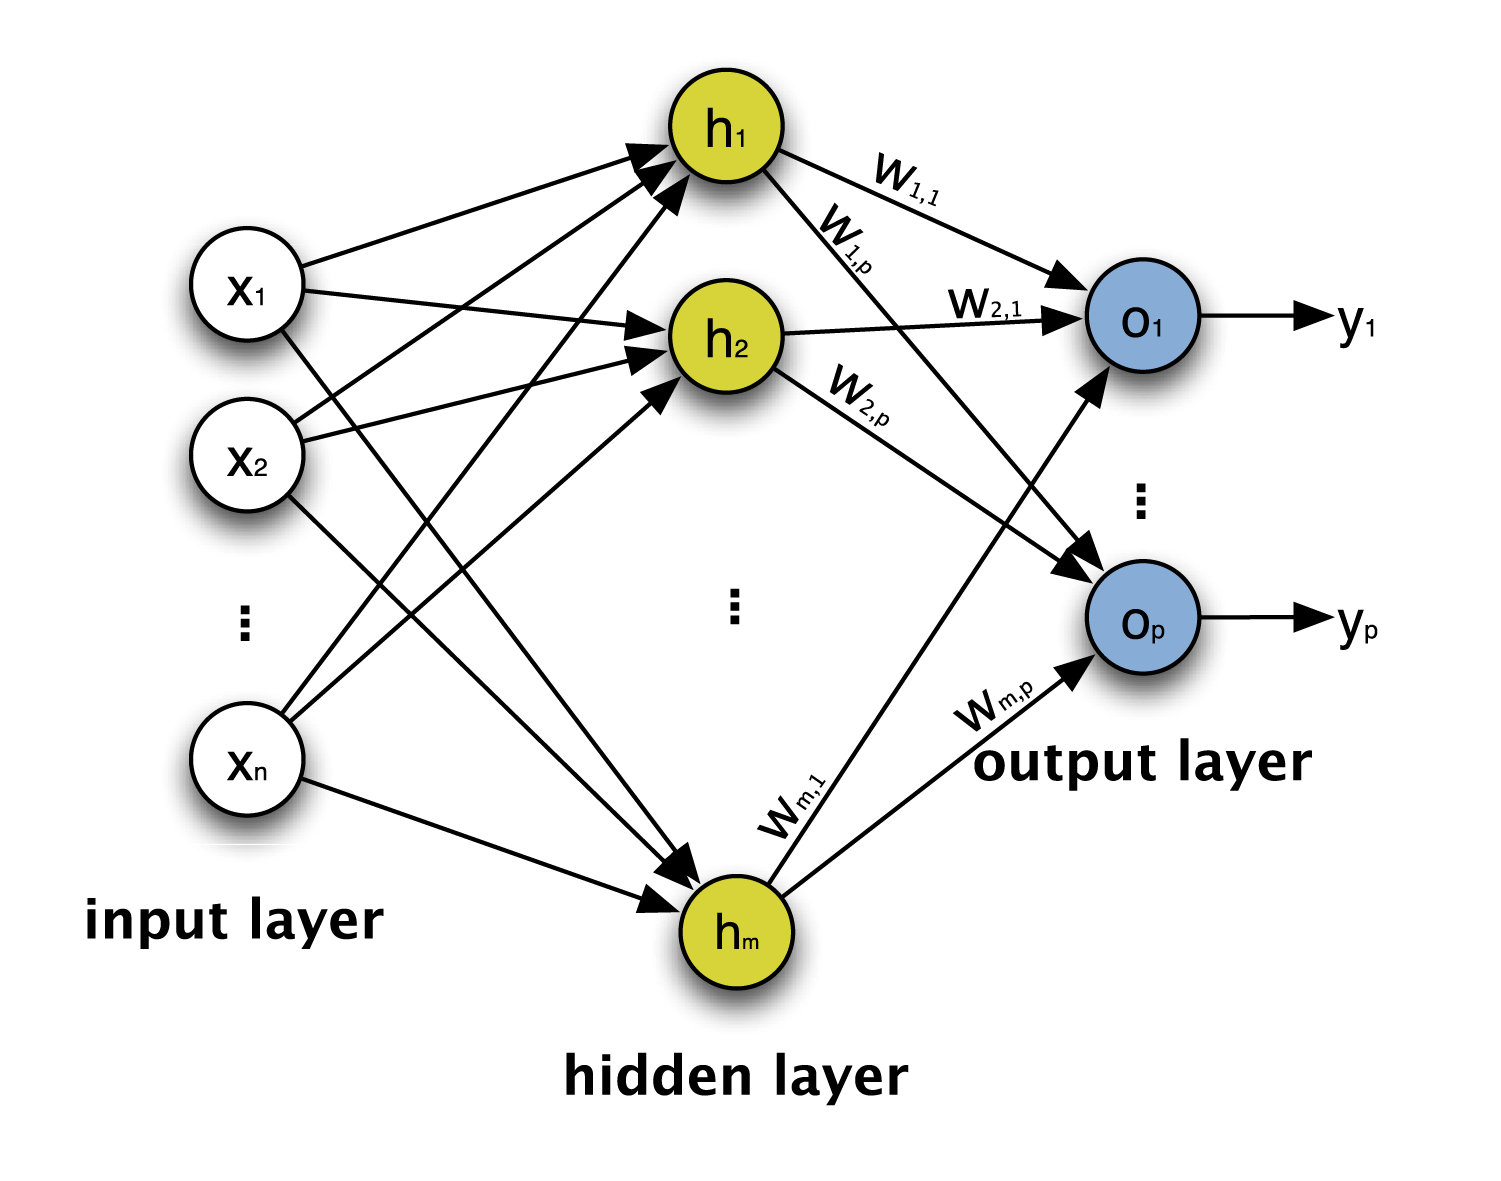
\includegraphics[width=0.5\textwidth]{img/rbf.png}
%	\end{center}
%	\legend{Fonte: elaborado pelo autor}
%\end{figure}
Os dados de entrada geralmente constituem em um vetor cujos elementos são pesos para cada uma das características da amostra.  A classificação das entradas com base no vetor de características é feito por meio de uma função de ativação sendo que cada tipo de RNA apresenta diferentes métodos de acordo com sua arquitetura. 

Dentre os vários tipos de redes neurais existentes, podemos citar as Redes Neurais de Base Radial (\textit{Radial Basis Function - RBF}), Redes Neurais do tipo Perceptron Multi-camadas (\textit{Multilayer Perceptron - MLP}) Redes Neurais Probabilísticas (\textit{Probabilistic Neural Networks - PNNs}) \cite{specht1990} \cite{specht1992}. Por possuírem uma arquitetura mais simplista, as RBFs tem sido objeto de estudo de diversos trabalhos, bem como as PNNs e suas versões melhoradas. 

A aplicação de RNAs no contexto de balanceamento de cargas é ainda pouco explorado e pode apresentar bons resultados. Como o balanceamento de carga em sistemas de nuvem dependem, de certa forma, das características do serviço e/ou da requisição, o presente projeto propõe uma abordagem no contexto apresentado utilizando RNAs. Tendo estes conceitos em vista, o presente projeto tem por objetivo um protótipo de aplicação de RNAs no balanceamento de carga em sistemas em nuvem. 


% ---
% Objetivos
% ---
\section{Objetivos}\label{cap:objetivos-justificativa}
% ---

% ---
% Objetivos Gerais
% ---
\subsection{Objetivos Gerais}\label{sec:objetivos-gerais}
% ---

O objetivo geral deste projeto é planejar e desenvolver um módulo de aplicação que utiliza uma rede neural artificial no balanceamento de carga em serviços de nuvem, bem como analisar seu uso em ambientes reais.

% ---

% ---
\subsection{Objetivos Específicos}\label{sec:objetivos-especificos}
% ---

\begin{alineas}
	\item Estabelecer o estado da arte acerca de aplicação de redes neurais artificiais no contexto de balanceamento de carga em sistemas de nuvem;
	\item Estudar o funcionamento de serviços em nuvem;
	\item Identificar características e requisitos considerados no balanceamento de carga;
	\item Definir os elementos necessários para desenvolvimento da aplicação que fará o balanceamento;
	\item Definir tipo de RNA a ser utilizada;
	\item Planejar a estrutura da aplicação;
	\item Implementar a ferramenta inteligente;
	\item Analisar os resultados no contexto de balanceamento de carga;
\end{alineas}

% ---
% ---------------------------------------------------------- % inclui o arquivo introducao.tex

% ----------------------------------------------------------


% ----------------------------------------------------------
% Fundamentação Teórica
% ----------------------------------------------------------

% ----------------------------------------------------------
% Fundamentação Teórica
% ----------------------------------------------------------
\chapter{Fundamentação Teórica}\label{cap:fundamentacao-teorica}
% ----------------------------------------------------------
Nesta seção apresentam-se conceitos, fundamentos e teorias que dão suporte ao presente trabalho. Dentre eles, Computação em Nuvem, Balanceamento de Cargas e Redes Neurais Artificiais.
% ---
\section{Computação em Nuvem}\label{sec:cloud-comp}
% ---
Computação em Nuvem ou \textit{Cloud Computing} refere-se tanto à aplicações entregues como serviços via Internet quanto ao \textit{hardware} e sistemas de \textit{software} em \textit{data centers} que provém tais serviços \cite{Armbrust:2010}. Atualmente, serviços em nuvem tem criado novas oportunidades por oferecerem serviços a valores mais acessíveis para empresas de diversos tamanhos. Nos últimos anos, os benefícios econômicos tem se tornado evidentes tanto pela aceitação deste conceito, quanto pela adesão das empresas ao modelo de Computação em Nuvem \cite{raza2015}.

A Computação em Nuvem pode ser definida como um “modelo que permite acesso a rede de forma ubíqua, conveniente, \textit{on-demand} para compartilhar um grupo de recursos computacionais configuráveis (como por exemplo rede, servidores, armazenamento, aplicações e serviços) que podem ser rapidamente fornecidos e gerados com mínimo esforço de gerenciamento ou interação com o provedor”\cite{mell2011nist}. Ainda segundo Mell (2011), para ser considerado um modelo em nuvem, uma plataforma de Computação em Nuvem deve atender as características essenciais, a saber: 
\begin{alineas}
	\item \textit{On-demand self-service}, definido como a capacidade do usuário de autorregular características como armazenamento de acordo com sua necessidade e de forma automática;
	\item \textit{Broad network access}, que define a disponibilidade de acesso através da rede utilizando dispositivos diversos; 
	\item \textit{Resource pooling}, fornecimento dos serviços a múltiplos usuários, associando dinamicamente recursos heterogêneos de acordo com a demanda solicitada. Há ainda um senso de independência, visto que o usuário geralmente não possui conhecimento ou controle sobre a localização física do recurso, devido ao alto nível de abstração; 
	\item \textit{Rapid elasticity}, referente a capacidades relacionadas a elasticidade de fornecimento e alocação, em alguns casos automática, para garantir escalabilidade, dando a impressão de um serviço com capacidades ilimitadas; 
	\item \textit{Measured service}, referente ao controle e otimização automática de recursos usados aproveitando a capacidade de medição no nível de abstração apropriado para o tipo de serviço (como por exemplo armazenamento, processamento, largura de banda e número de usuários ativos). Recursos podem ser monitorados e controlados, o que garante a transparência tanto para o fornecedor do serviço quanto para o consumidor. 		
\end{alineas}

\subsection{Modelos de Computação em Nuvem e Tipos}\label{sec:mod}

Além das características essenciais, há também a separação por tipos de serviço. Neste caso, o tipo de serviço em nuvem é dividido com base em como funciona o fornecimento do serviço, bem como qual o nível de abstração atendido por aquele serviço, tal como apresentado na Figura 1. Neste sentido, há três tipos de separação: 

\begin{figure}[htb]
	\caption{\label{fig:cloud_en}Modelos de Computação em Nuvem}
	\begin{center}
		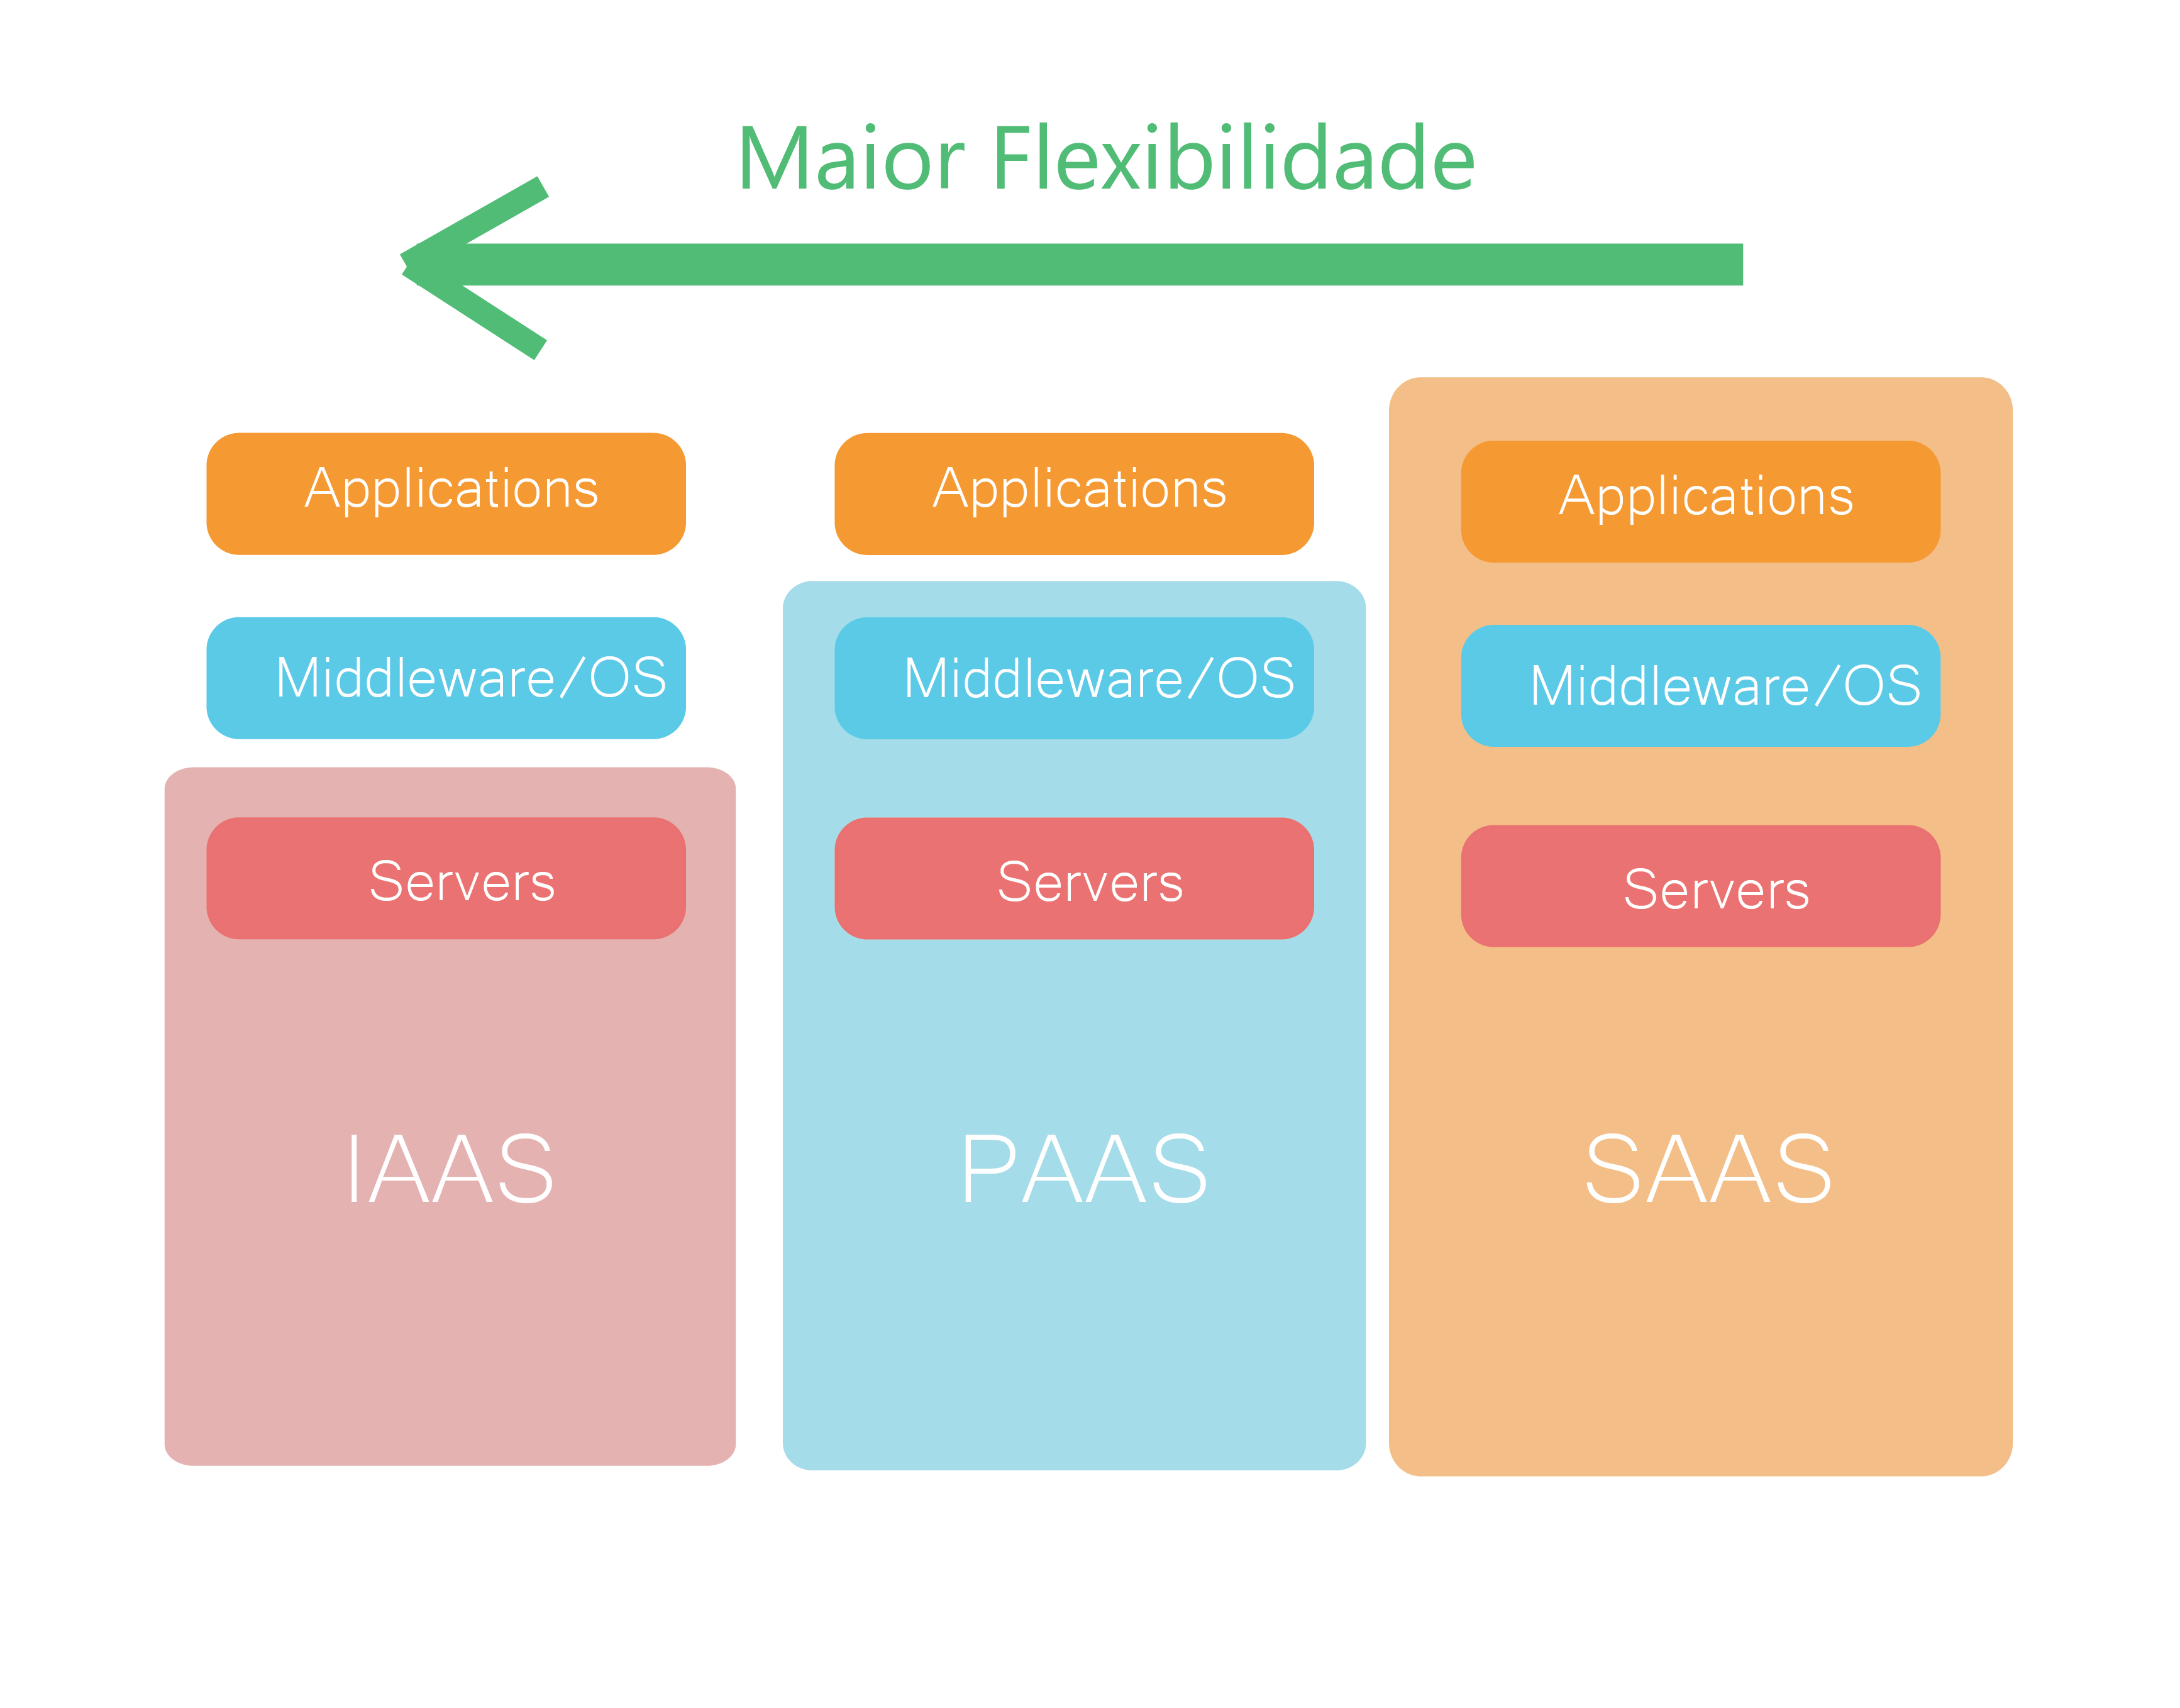
\includegraphics[width=0.50\textwidth]{img/cloud_en.png}
	\end{center}
	\legend{Fonte: \citeonline{pbxl}}.
\end{figure}


\textit{Software as a Service (SaaS)}: modelo no qual o consumidor utiliza o serviço fornecido por uma aplicação executada em uma infraestrutura de nuvem, sendo que esta aplicação fica acessível a partir de vários dispositivos do tipo cliente, através de uma interface que pode ser um navegador web ou programa. Neste caso especificamente, o cliente não gerencia a infraestrutura da nuvem, tampouco da aplicação utilizada \cite{mell2011nist}. 

\textit{Platform as a Service (PaaS)}: este modelo permite que se tenha acesso a uma plataforma com infraestrutura de nuvem onde o usuário pode criar aplicações utilizando linguagens de programação, bibliotecas, serviços e ferramentas suportadas pelo fornecedor do serviço. O usuário não gerencia ou controla camadas mais baixas da infraestrutura tais como servidores, sistema operacional ou armazenamento, embora seja responsável pela aplicação e pelo ambiente servidor da mesma\cite{mell2011nist}. Como exemplo dessa plataforma é possível citar o Windows Azure \cite{Azure}

\textit{Infrastructure as a Service (IaaS)}: a oferta de infraestrutura como serviço é o menos abstrato dos modelos. Neste caso o usuário tem a capacidade de gerenciar recursos fundamentais tais como sistema operacional e demais aplicações. Embora não tenha controle sobre a camada de \textit{hardware} da infraestrutura da nuvem, ele pode controlar recursos de sistema, armazenamento e instalar aplicações e, em alguns casos, até ter certo controle sobre certos componentes de rede, como \textit{firewalls}\cite{zhang2010cloud}. Como exemplo de fornecedores de serviço em nuvem que seguem esse modelo temos a \textit{Amazon EC2}\cite{AmazonEC2}. 

Além da identificação do modelo há também a separação por tipos \cite{zhang2010cloud}. Geralmente, são divididos em três: públicas, privadas e híbridas. Nuvens públicas tem como característica principal oferecer serviços para o público em geral, sendo gerenciadas por uma organização. Nuvens privadas possuem infraestrutura fornecida e gerenciada por uma organização proprietária da nuvem, sendo gerenciada e operada pela mesma. Nuvens híbridas, por sua vez, são compostas por duas ou mais infraestruturas distintas (privada e pública, por exemplo), que, embora mantenham suas características, são ligadas de alguma maneira habilitando a portabilidade entre elas\cite{mell2011nist} \cite{zhang2010cloud} \cite{Bhaskar}.

Atualmente, há diversas plataformas e empresas que fornecem \textit{softwares} e serviços para habilitar a Computação em Nuvem, seja em nuvens públicas, privadas ou híbridas. Há também uma grande quantidade de modelos, tipos e serviços de maneira acessível. 
\newline

% ---
\textbf{\textit{{AWS - Amazon Web Services}}}

A \textit{{AWS - Amazon Web Services}} consiste em uma plataforma que fornece diversos serviços em nuvem, incluindo infraestrutura sob demanda para computação de alto desempenho, armazenamento, aplicações, dentre outros recursos.\cite{AmazonSolutions}. A AWS oferece serviços que vão desde serviços para computação, como por exemplo a EC2\cite{AmazonEC2}, passando por armazenamento e bancos de dados \cite{AmazonDB}, até ferramentas para infraestruturas de Internet das Coisas (IoT)\cite{AmazonIoT}. 
\newline

% ---
\textbf{\textit{{CloudStack}}}

% ---
O Apache CloudStack é um \textit{software} \textit{open source} desenvolvido para instalar e gerenciar redes de máquinas virtuais baseados em IaaS para plataformas em nuvem. Contém diversos serviços públicos, podendo ser utilizado em conjunto com nuvens privadas, gerando estruturas híbridas. Sua funcionalidade mais procurada é a possibilidade de utilizar a rede como um serviço, pela facilidade de controle e gerenciamento. 
\newline

% ---
\textbf{Outras Plataformas e \textit{Softwares}}

% ---
Atualmente há um grande número de plataformas e empresas que fornecem serviços de computação em nuvem, como por exemplo a Microsoft (Azure), IBM (IBM Cloud) e Google (Google Cloud Platform), Eucalyptus, dentre outras.


% ---
\section{Balanceamento de Carga}\label{sec:balanceamento-carga}
% ---

Balanceamento de Carga ou \textit{Load Balancing} consiste em transformar uma grande carga de processamento em cargas menores com o intuito de aumentar o desempenho do sistema através da distribuição entre nós desse sistema. Em um ambiente de computação em nuvem, o balanceamento de cargas é necessário para realizar de maneira dinâmica a distribuição local da carga de maneira igualitária, entre todos os nós\cite{kaur2012load}. Cabe ressaltar que os nós de uma nuvem referem-se a infraestrutura de \textit{hardware} distribuída em localidades distintas e transparentes ao usuário. A Figura 2 representa uma estrutura simplificada de como funciona o balanceamento de carga. 

\begin{figure}[htb]
	\caption{\label{fig:bal}Estrutura Simplificada de Balanceamento de Carga}
	\begin{center}
		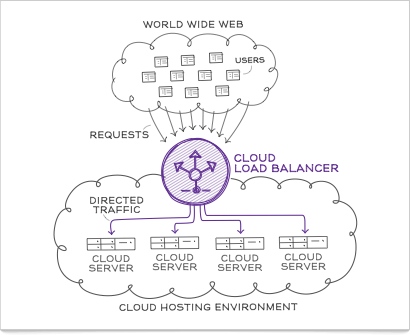
\includegraphics[width=0.50\textwidth]{img/cloud_balancer.png}
	\end{center}
	\legend{Fonte: \citeonline{rack}}
\end{figure} 

Tal conceito se torna essencial quando aplicado a computação em nuvem, uma vez que esse tipo de modelo depende necessariamente da disponibilidade e do tempo de resposta. Isto, acrescido dos conceitos essenciais para Computação em Nuvem apresentam o balanceamento de carga como um problema que requer atenção no contexto de computação em nuvem \cite{sran2013comparative}. Assim, a distribuição de carga através da nuvem impacta diretamente no desempenho geral do sistema. 

Identificar os desafios encontrados no balanceamento de carga em sistemas de nuvem é um dos caminhos para entender quais características um algoritmo de balanceamento de carga deve funcionar de modo satisfatório. Segundo \citeonline{surveycloud:2012}, pode-se citar os seguintes tópicos: 

\begin{itemize}
	\item distribuição esparsa dos nós da nuvem: consiste em um desafio visto que criar um algoritmo capaz de funcionar em arquiteturas esparsas e altamente distribuídas torna-se difícil, visto que é preciso levar em consideração a distancia entre os nós e consequentemente, adequar o algoritmo a atrasos; 
	
	\item armazenamento/replicação: a replicação de dados entre os nós pode resultar em maior custo, uma vez que mais capacidade de armazenamento é requerida;
	
	\item complexidade do algortimo: é preferível que algoritmos de balanceamento não sejam tão complexos em termos de implementação, pois isto pode resultar em requisições maiores de informação aumentando o tempo de resposta, o que diminui a eficiência; 
	
	\item ponto de falha: a coleta de dados acerca das informações sobre nós diferentes deve ser projetada com o intuito de evitar erros no algoritmo. Geralmente algoritmos centralizados tendem a ser mais eficientes para certos tipos de arquiteturas, mas costumam falhar em outras. Algoritmos distribuídos, por sua vez, possuem uma abordagem melhor, mas mais complexa.
\end{itemize}

Os algoritmos de balanceamento de carga podem ser divididos, de forma generalizada, em estáticos - associa cargas com base na habilidade do nó de processar tarefas, sem levar em consideração mudanças em tempo real - e dinâmicos - considera diferentes aspectos dos nós, incluindo capacidade e largura de banda \cite{surveycloud:2012}. 

É importante ressaltar que o balanceamento preferivelmente deve ser feito de forma dinâmica, visto que o comportamento da nuvem pode variar e a infraestrutura geralmente é composta de \textit{hardwares} distintos. Além disto, a distribuição de carga busca melhorar a eficiência de sistemas distribuídos considerando questões que ainda apresentam-se como desafios na área de computação em nuvem, tais como gerenciamento eficiente de tráfico, gerenciamento de energia e alocação dinâmica de recursos\cite{zhang2010cloud}. Tendo isto em vista, existem critérios que devem ser considerados na definição das métricas que quantificam a efetividade de algoritmos de balanceamento. Ainda segundo \citeonline{surveycloud:2012}, podemos citar os seguintes critérios: 

\begin{enumerate}
	\item taxa de transferência - relacionado ao número de tarefas completadas; 
	\item custo associado ao algoritmo de balanceamento; 
	\item tolerância a falhas;
	\item tempo de resposta; 
	\item escalabilidade e flexibilidade na capacidade de distribuição das cargas de acordo com a demanda, bem como se adequar rapidamente às demandas; 
	\item utilização de recursos;
	\item desempenho do sistema. 	
\end{enumerate}


Pode-se considerar que os objetivos do balanceamento de carga são, de maneira geral, melhorar o desempenho do sistema a um custo mais baixo; garantir a escalabilidade e flexibilidade, de forma que o algoritmo se adapte facilmente à possíveis mudanças no sistema e, por fim, garantir que a prioridade (caso haja) seja respeitada\cite{kaur2012load}. 

Diversos algoritmos de balanceamento foram propostos, com abordagens distintas, mas sempre tentando atender da melhor forma possível os objetivos de balanceamento de carga. Dentre eles pode-se citar o \textit{Round Robin} \cite{soni2014novel}, \textit{Biased Random Sampling} \cite{randles2010comparative1}, \textit{Active Clustering} \cite{randles2010comparative1}, \textit{Ant Colony}\cite{nishant2012load} e \textit{Honeybee Foraging Behavior} \cite{randles2010comparative1}.  

\newpage
% ---
\section{Redes Nerais Artificiais}\label{sec:rna}
% ---

Técnicas de reconhecimento de padrões tem por objetivo aprender funções de decisão que separam um conjunto de dados em agrupamentos de amostras (\textit{clusters}) que compartilham propriedades similares\cite{Duda:00}. Tal processo de aprendizado de funções de decisão podem ser geralmente associados a três abordagens: (i) supervisionada, na qual, a princípio, se conhece informações sobre todo o conjunto de treinamento; (ii) semi-supervisionado, no qual parte das informações sobre o conjunto de treinamento é conhecido e (iii) não-supervisionado, no qual não se tem informações prévias a respeito das amostras do conjunto de treinamento. 

Técnicas supervisionadas são conhecidas por apresentarem melhores taxas de acurácia, uma vez que a quantidade de informações disponíveis acerca das amostras de treinamento permite que tais técnicas aprendam a classificar de maneira específica determinadas propriedades, bem como permite a construção de estruturas mais complexas de aprendizagem de forma a aprimorar a qualidade do processo de treinamento.

O estado da arte neste campo tem como referência técnicas como Máquinas de Vetores Suporte (\textit{Support Vector Machines – SVM}), proposta por \citeonline{cortes1995support}, Redes Neurais (\textit{Neural Networks}), amplamente discutidas por Haykin (2007), classificadores Bayesianos e os amplamente conhecidos k-médias ( \textit{k-nearest neighbours – k-NN}), dentre outros\cite{Duda:00}. 

Dentro do contexto de reconhecimento e classificação de padrões, as Redes Neurais Artificiais tem sido amplamente estudadas em diferentes contextos de aplicações. Há, atualmente, diversos tipos de configurações de arquiteturas destas redes. De forma geral, sua arquitetura é formada por camadas de neurônios, sendo a configuração mais trivial composta por uma camada de entrada (\textit{input layer}), uma ou mais camadas escondidas (\textit{hidden layer}) e uma camada de saída (\textit{output layer}). Cada neurônio em sua respectiva camada recebe um estímulo que é processado pelo neurônio e propagado à camada seguinte, como representado na figura 3. 
\begin{figure}[ht!]
	\caption{Estrutura de uma ANN}
	\label{fig:ann-arq}
	\begin{center}
		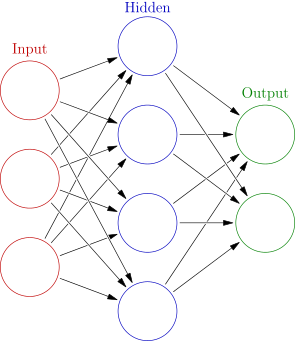
\includegraphics[scale=0.48]{img/ann-arq.png}
	\end{center}
	\legend{Fonte: \citeonline{wiki}}
\end{figure}

As Redes Neurais Artificiais ou \textit{Artificial Neural Networks - ANN} são compostas por elementos chamados neurônios, os quais, segundo \citeonline[p.~11]{Haykin2ndnew}, são unidades de processamento que ao receber um valor de entrada (ou \textit{input}) são responsáveis por processá-lo e propagar o sinal para a próxima camada. Este processamento pode ocorrer, basicamente, de três formas diferentes: 
\begin{itemize}[noitemsep]
	\item multiplicação da entrada por um peso; 
	\item o neurônio funciona tal qual um somador, ou combinador linear de suas entradas;
	\item o sinal de entrada é parâmetro de uma função de ativação responsável por limitar a amplitude do sinal de saída, como ocorre em uma sigmoide, por exemplo.
\end{itemize}

Dentro deste contexto, há atualmente uma diversidade muito grande de arquiteturas nas quais é possível organizar essas pequenas unidades. O poder de aprendizado das redes neurais permite efetuar desde tarefas mais simples, até atuar em complexos sistemas de aprendizado e classificação, como por exemplo, no reconhecimento de imagens e voz - basta ver exemplos como os das Redes Neurais Recorrentes (\textit{Recurrent Neural Networks - RNN})\cite{rnn} ou Redes Neurais de Convolução (\textit{Convolutional Neural Networks - CNN}). Dentre as aplicações de ANNs, podemos citar o uso no controle, classificação, previsão, como filtros para extrair informações, dentre outras. 

No entanto, nem todos os problemas exigem arquiteturas tão complexas. Segundo \citeonline[p.~21-23]{Haykin2ndnew}, há três tipos fundamentais de estruturas: \textit{Single Layer Feedfoward Networks} (Redes Neurais de Camadas Únicas), \textit{Multilayer Feedfoward Networks} (Redes com Múltiplas Camadas) e \textit{Recurrent Networks} (Redes Neurais Recorretes).

\begin{figure}[ht!]
	\caption{Fluxo de aprendizado de uma rede neural}
	\label{fig:annfluxo}
	\begin{center}
		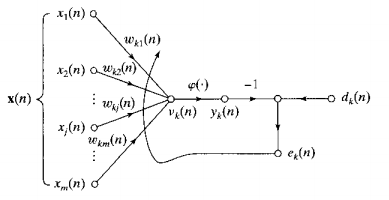
\includegraphics[scale=0.8]{img/annflowlearning.png}
	\end{center}
	\legend{Fonte: \citeonline[p.~52]{Haykin2ndnew}}
\end{figure}

É importante ressaltar que a quantidade de camadas em uma rede impacta diretamente no desempenho em relação ao processamento e na velocidade de aprendizado. Além disso, a escolha de implementações de arquiteturas que atendam à um problema específico ou sejam demasiadamente especializadas não é recomendado pois pode tornar a arquitetura ineficiente na resolução de problemas diferentes daqueles na qual foi treinada. 

\subsection{Perceptron}

Perceptrons de única camada são uma alternativa simples de implementação de rede neural para identificar dados que são linearmente separáveis. O conceito aplicado é de uma rede que recebe vetores de características que treinam o Perceptron para identificar padrões e classificar amostras. Um neurônio também forma uma base de um filtro adaptativo, que pode ser aplicado em um sistema dinâmico. De forma geral, a Figura \ref{fig:annfluxo} representa a propagação de sinal por um modelo adaptativo. No caso de um Perceptron, a propagação de sinal é feita por meio de uma função não-linear. A representação do fluxo de sinal de um Perceptron, ilustrado na Figura \ref{fig:perceptron}, denota exatamente este fluxo de processamento. 
	
\begin{figure}[ht!]
	\caption{Fluxo de sinal em um Perceptron}
	\label{fig:perceptron}
	\begin{center}
		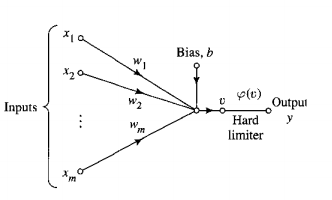
\includegraphics[scale=0.8]{img/perceptron.png}
	\end{center}
	\legend{Fonte: \citeonline[p.~136]{Haykin2ndnew}}
\end{figure}	

O Perceptron tem em seu modelo um fluxo (representado na figura \ref{fig:perceptron}) no qual os pesos $w_1, w_2, ... , w_m$ são sinapses do Perceptron, correspondentes à cada uma de suas respectivas entradas, denotadas por $x_1, x_2, ... , x_m$. Uma \textit{bias} pode ser aplicada externamente, denotada por $b$. O nó $ v $ recebe a propagação do sinal e, a partir da aplicação de uma função propaga a saída $y$ (\textit{Output}). A partir do modelo, pode-se inferir que o limitador da camada de entrada, ou local de indução dos neurônios é denotado pela equação \ref{eq:funcperceptron}.  

\begin{equation}
v = \sum_{i=1}^{m} ({w_i} \times {x_i} + b)
\label{eq:funcperceptron}
\end{equation}

O objetivo de um Perceptron, de forma geral, é classificar corretamente a entrada, ou seja, $x$ em uma de duas classes, $C_1$ ou $C_2$. Neste contexto, a regra de decisão associa o ponto representado pelo vetor $x$ em uma das classes, dada sua saída. Os pesos em $w$ podem ser ajustados a cada iteração e, para isso, usa-se uma função de ajuste, seja por correção de erro, seja por regras de convergência \citeonline{Haykin2ndnew}. Nesse caso, um dos algoritmos que pode ser seguido está representado a seguir:
\begin{enumerate}
	\item \textit{inicialização de paramêtros}: inicialização do vetor de pesos (lembrando que a atualização é feita em $n$ \textit{steps} ou iterações);
	\item \textit{ativação}: em cada \textit{step}, receber a entrada (ou \textit{input}) e ativar o Perceptron;
	\item \textit{computar a saída}: resposta do perceptron $y(n)$, ou seja, a saída da função de ativação;
	\item \textit{ajuste}: ajuste dos pesos de $w$ 
	\item \textit{continuação}: repetição do processo	 
\end{enumerate}

\subsection{\textit{ANNs} com Múltiplas Camadas}



Como variação do Perceptron tem-se uma rede de múltiplas camadas, chamada Perceptron Multicamada (PMC), que são constituídas de um conjunto de neurônios sensoriais que formam uma camada de entrada, uma ou mais camadas ocultas de nós computacionais e uma camada de saída, também com nós computacionais. O sinal de entrada, recebido pela camada de entrada, é propagado para a próxima camada, repetindo esse processo até a camada de saída\citeonline[p.~98]{Haykin98p93}. 

Cada neurônio possui uma função de ativação, geralmente não-linear. A não linearidade dessa função é importante para a saída da rede, visto que permite que valores de classificação não binária sejam atribuídos, o que permite que haja classificação de duas ou mais classes. A camada escondida capacitam a rede a aprender tarefas complexas extraindo progressivamente as características mais significativas. A Figura \ref{fig:pmc} apresenta a estrutura generalizada de um Perceptron Multicamadas. 

\begin{figure}[ht!]
	\caption{\label{fig:pmc}Estrutura de um Perceptron Multicamada}
	\begin{center}
		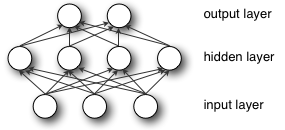
\includegraphics[width=0.5\textwidth]{img/mlp.png}
	\end{center}
	\legend{Fonte: \citeonline{mlp}}
\end{figure}

Redes Neurais de Base Radial (\textit{Radial Basis Function - RBF}) é uma rede neural semelhante ao PMC constituída por no mínimo três camadas, sendo uma de entrada, uma escondida e uma de saída. Nesta rede, a camada de entrada recebe um vetor de características ao qual é aplicada uma transformação não-linear na camada escondida. A Figura \ref{fig:rbf2} apresenta a estrutura de uma RBF genérica. 

\begin{figure}[htb]
	\caption{\label{fig:rbf2}Estrutura de uma Rede Neural com função de Base Radial}
	\begin{center}
		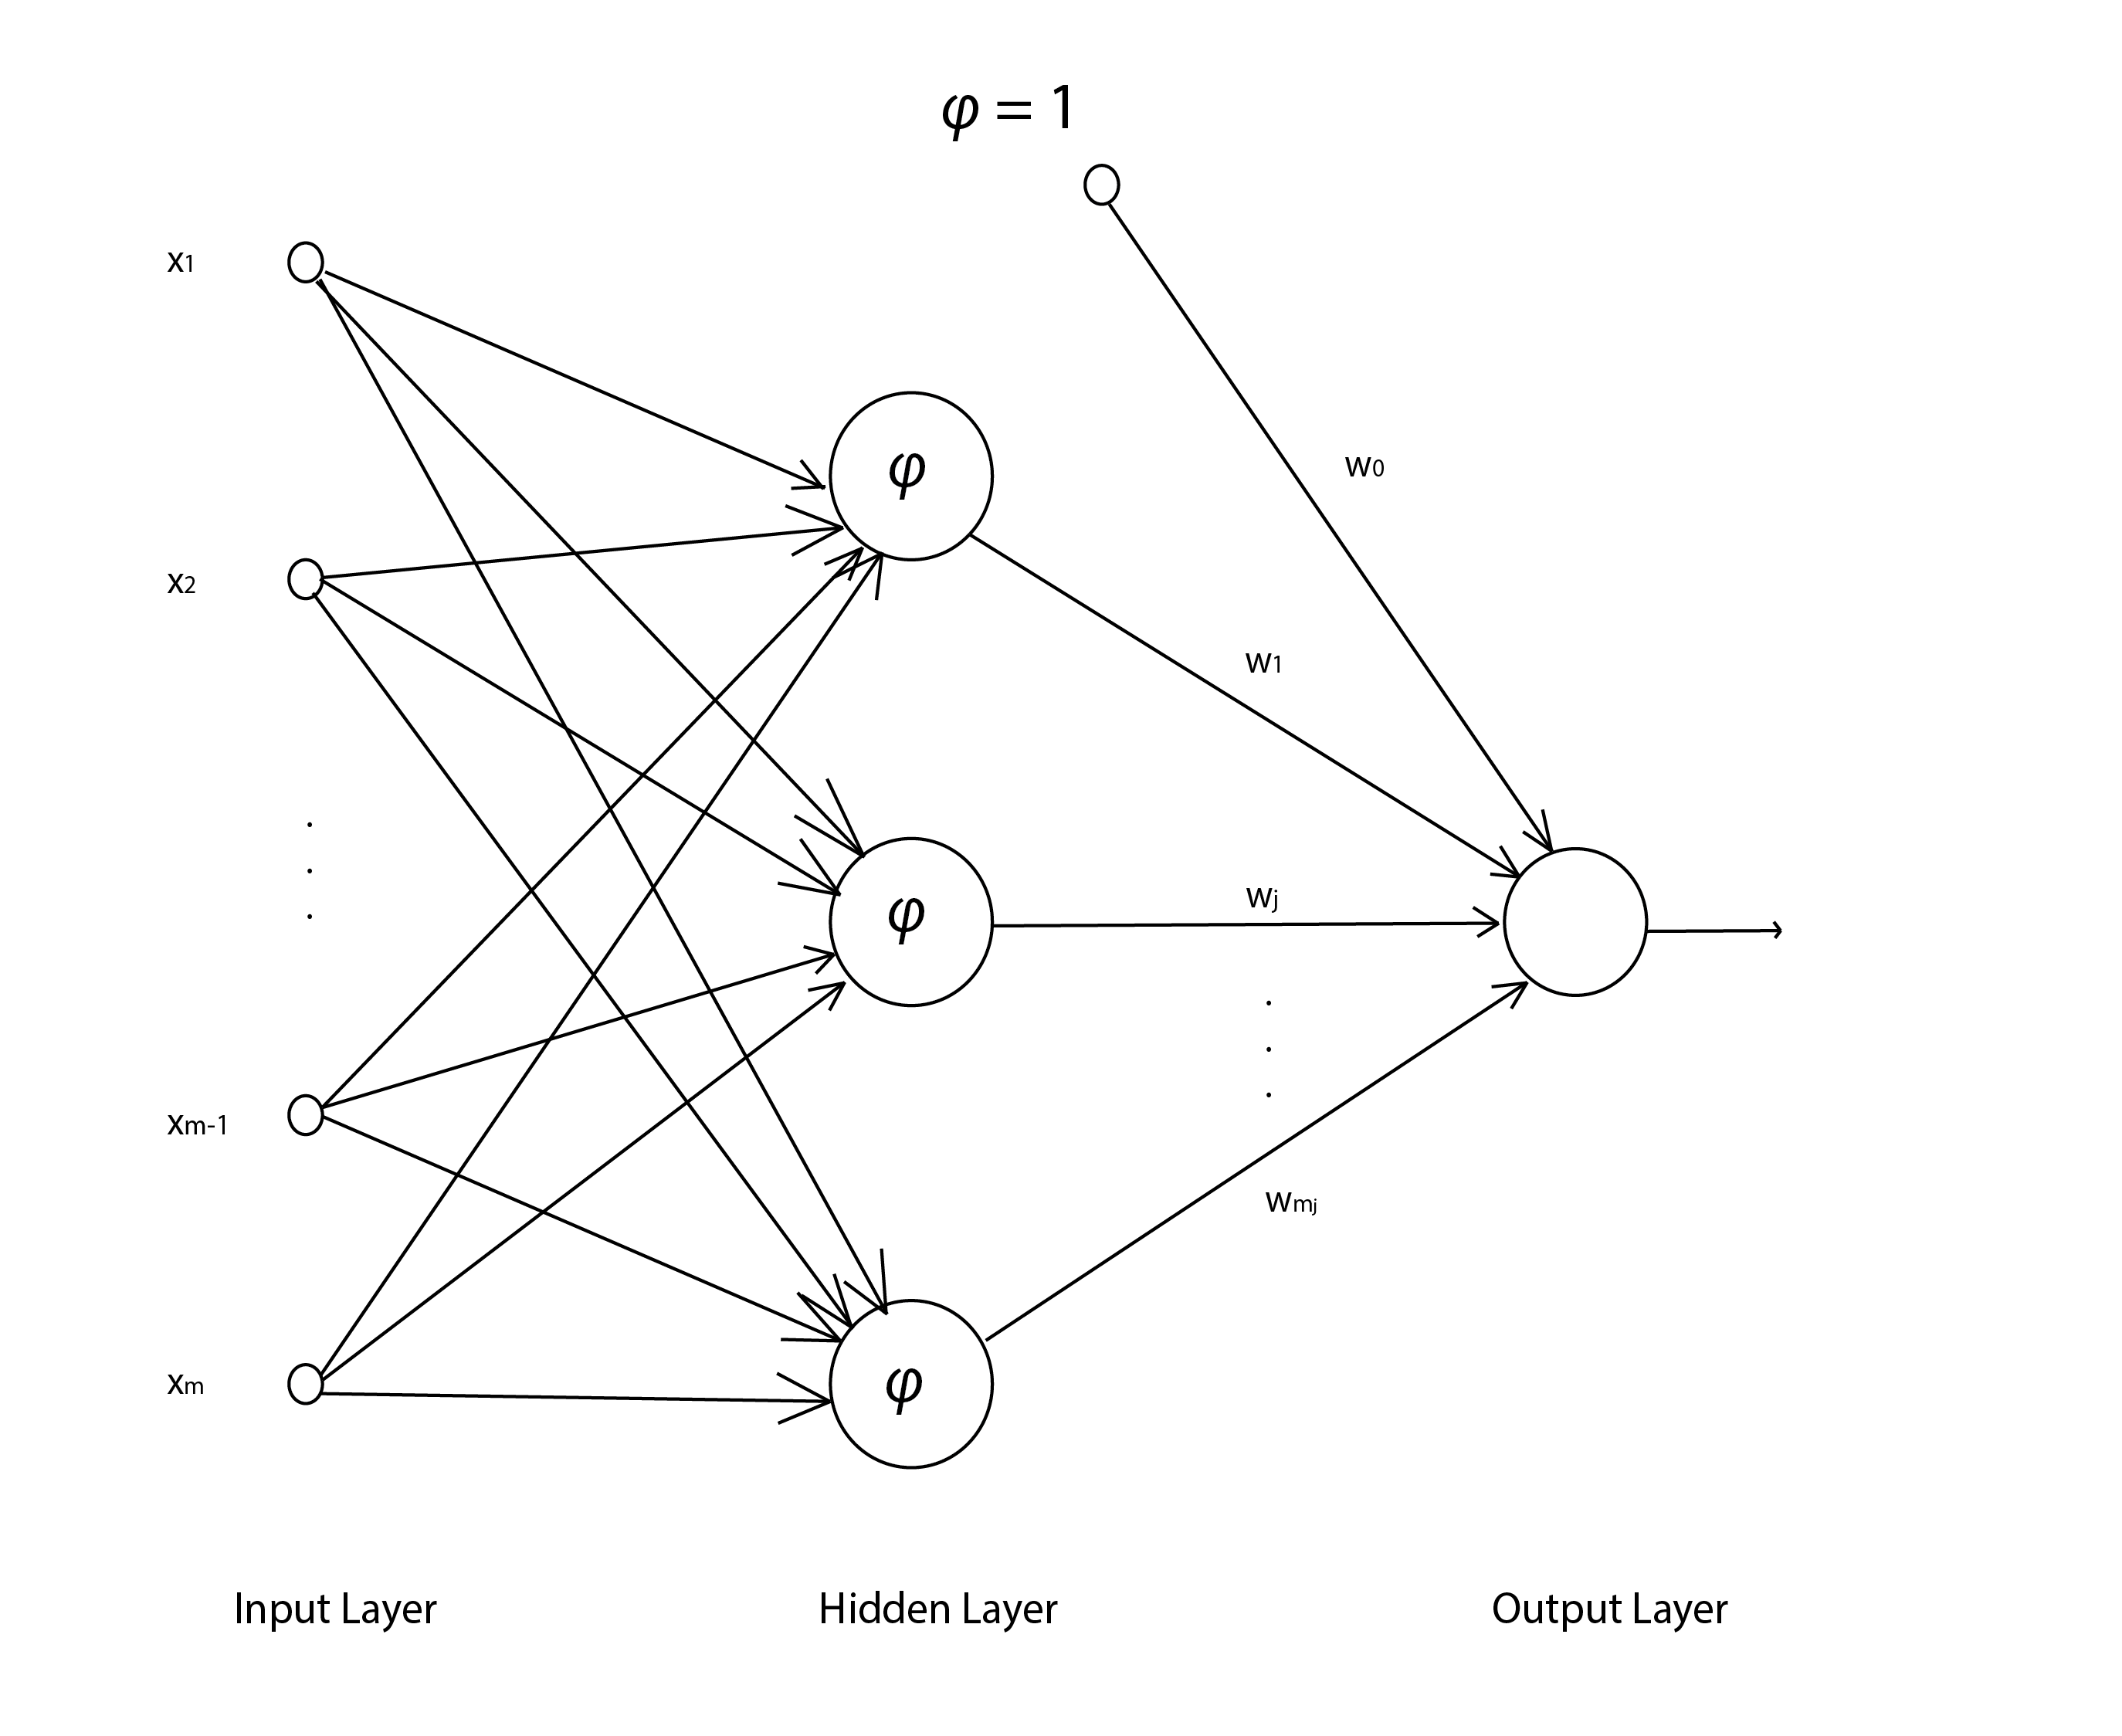
\includegraphics[width=0.60\textwidth]{img/rbf2.png}
	\end{center}
	\legend{Fonte: Baseado em \citeonline[p.~278]{Haykin2ndnew}}
\end{figure}

O diferencial da RBF para o PCM é, além da estrutura, a função de ativação aplicada para aprender as características mais relevantes. Neste caso, a função de ativação mais empregada é a Gaussiana, por sua formulação simples. 

Existem outros tipos de redes,tais quais as Redes Neurais Probabilística (\textit{Probabilistic Neural Network - PNN})\cite{specht1990probabilistic}, que funcionam de maneira semelhante a uma RBF. Sua camada escondida, no entanto, e dividida em duas partes: uma camada de padrões e uma camada de somatório. A Figura 6 apresenta a estrutura generalizada de uma PNN. A primeira tem por objetivo calcular a probabilidade de um determinado vetor de característica \textit{y} pertencer à uma classe \textit{x}. A segunda camada, por sua vez, realiza um somatório dessas probabilidades. Na camada de saída, os dados recebidos da camada anterior são utilizados para classificar as amostras, atribuindo a \textit{y} o rótulo correspondente ao neurônio com maior probabilidade.

% ---------------------------------------------------------- % inclui o arquivo fundamentacao.tex

% ----------------------------------------------------------


% ----------------------------------------------------------
% Metodologia
% ----------------------------------------------------------

% ----------------------------------------------------------
% Metodologia
% ----------------------------------------------------------
\chapter{Metodologia}\label{cap:metodologia}
% ----------------------------------------------------------
Neste capítulo estão descritos as ferramentas e metodologia utilizadas para o desenvolvimento do projeto, além da apresentação da arquitetura do protótipo de balanceamento proposta. 

% ----------------------------------------------------------
\section{Tecnologias e Ferramentas Utilizadas}\label{sec:tecnologias-ferramentas}
% ----------------------------------------------------------
Nesta seção são apresentadas as ferramentas e tecnologias usadas na implementação do projeto. 

% ---
\subsection{AWS - \textit{Amazon Web Services}}\label{sec:aws}
% ---
A Amazon oferece um vasto portifólio de serviços baseados em Computação em Nuvem, concentrados na Amazon Web Services. Seus produtos variam desde a oferta de IaaS, com servidores virtuais, nuvens privadas, dentre outras ferramentas, até aplicações do tipo SaaS, como o serviço de armazenamento em nuvem (\textit{Amazon Cloud Drive}) \cite{AmazonCloudDrive}.

Sua plataforma de serviços web é centrada no Amazon Elastic Compute Cloud ou EC2. Trata-se de um “serviço que fornece capacidade de computação redimensionável na nuvem” \cite{AmazonEC2}. Por ter foco em desenvolvedores, possui uma interface com maior controle de recursos computacionais, incluindo configurações de memória, processamento, sistema operacional e armazenamento. Além disso, há suporte para outras ferramentas, como banco de dados, \textit{Big Data} e até mesmo Internet das Coisas. Além do baixo custo, uma das vantagens da Amazon está na flexibilidade dos planos de serviços, que são ajustáveis de acordo com a demanda \cite{AmazonEC2price}.

O acesso é feito por meio do AWS Management Console, que consiste em uma interface web para gerenciamento dos serviços. No caso da EC2, a visualização e acompanhamento de estado das instâncias é feito pela EC2 Dashboard, como exemplificado na figura \ref{fig:ec2con}. 

\begin{figure}[htb]
	\caption{\label{fig:ec2con}EC2}
	\begin{center}
		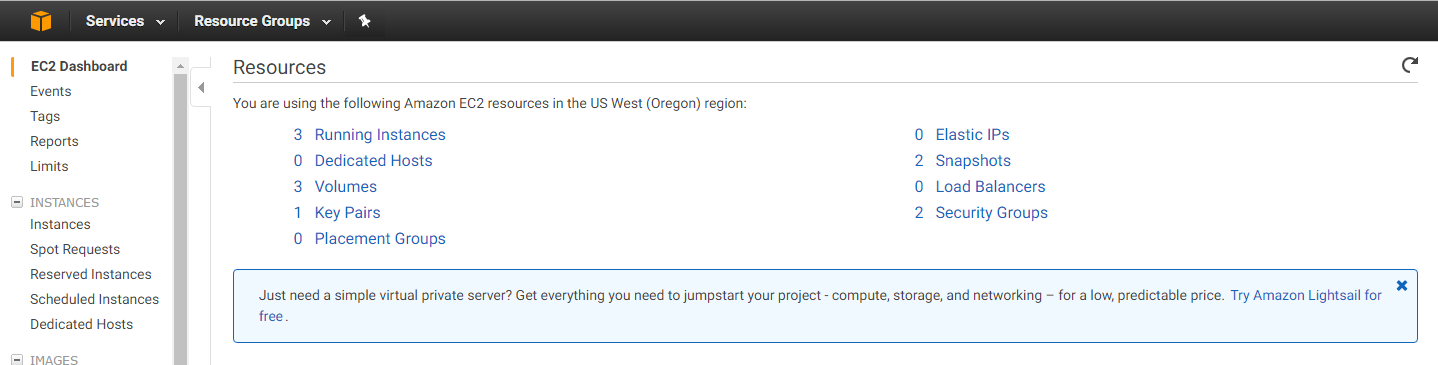
\includegraphics[width=0.90\textwidth]{img/ec2dash.png}
	\end{center}
	\legend{Fonte: elaborada pela autora}
\end{figure}

A AWS oferece diversos tipos de instâncias, as quais os tipos de uso variam de acordo com a aplicação. Instâncias do tipo T2, por exemplo, são indicadas para aplicações web, ambientes de desenvolvimento e teste e preparação de aplicações. Os preços também variam de acordo com o tipo de instância, uso e capacidade computacional \cite{amazon-cloud-instances}.Para este projeto, os servidores utilizados, bem como suas configurações estão descritos na tabela \ref{tab:servidores}. Todos as instâncias possuem como sistema operacional Ubuntu Server 16.04 LTS. 

	\begin{table}[h]
		\caption{Servidores}
		\centering
		\small
		\renewcommand{\arraystretch}{1.2} % Aumenta espaçamento vertical
		\begin{tabular}{c|c|c|c|c}
			\hline 
			\textbf{Servidor} & Tipo de instância & Memória & CPUs & Armazenamento \\ 
			\hline 
			\textbf{Servidor de balanceamento} & t2.medium & 4 & 2 & Somente EBS \\ 
			\hline 
			\textbf{Servidores do \textit{cluster} de aplicação} & t2.micro & 1 & 1 & Somente EBS \\ 
			\hline 
		\end{tabular}\\		
		\vspace{3mm}
		\legend{Elaborado pela autora.}
		\label{tab:servidores}
	\end{table}
	
Os servidores de requisição descritos na tabela \ref{tab:servidores} foram configurados para executar um código semelhante ao apresentado em \ref{sec:node-js} e são acessados apenas pelo servidor de balanceamento, através de seu DNS público, disponibilizado pela AWS para cada instância.  

% ---
\subsection{Node.js e npm}\label{sec:node-js}
% ---

Node.js\footnote{\url{https://nodejs.org/}} é uma plataforma de aplicações baseada no motor de Javascript do Google Chrome chamado V8\cite{nodejs}. Nessa plataforma, o Javascript que geralmente é utilizado no navegador, como forma de tornar dinâmica a interação do lado do cliente, é utilizado como linguagem para fornecer programação direta para o sistema operacional, permitindo a criação e execução no servidor. Seu código fonte está disponível\footnote{\url{https://github.com/nodejs/node}} para acesso, colaboração e comentários.
\begin{figure}[htb]
	\caption{\label{fig:codejs}Código exemplo de servidor em nodejs}
	\begin{center}
		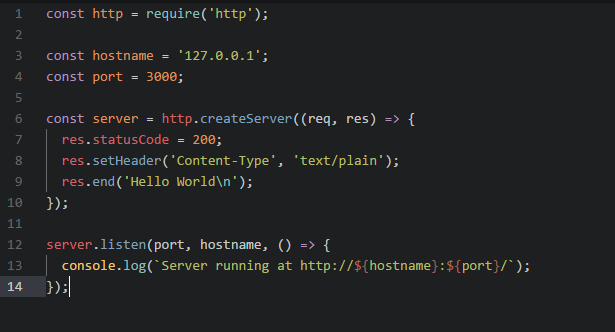
\includegraphics[width=0.50\textwidth]{img/codejs.png}
	\end{center}
	\legend{Fonte: elaborado pela autora}
\end{figure}
Essa plataforma funciona com base em um modelo voltado à eventos, ou seja, a execução não é bloqueada com eventos de entrada e saída (I/O), como nos demais modelos. O Node dispara funções específicas quando os eventos são acionados. Além disso, o Nodejs também possui um gerenciador de pacotes, o \textit{Node Package Manager} (denominado \textit{npm}). Seu objetivo é a instalação e distribuição de pacotes e bibliotecas criadas pela comunidade e que tenham código livre, o que permite que qualquer desenvolvedor disponibilize sua própria biblioteca.

Pacotes criados da maneira descrita anteriormente têm suas informações salvas em um arquivo chamado \textit{packages.json}, o qual contém informações como Nome do projeto, do criador, link para o repositório no GitHub, dependências de bibliotecas com a versão específica instalada, entre outros. Através do comando \textit{npm install} o gerenciador baixa e instala as dependências do módulo para executar a aplicação.A plataforma é acessível via terminal de comandos e está disponível para Windows, Mac OS e sistemas operacionais baseados em Linux. Neste projeto, a versão utilizada da plataforma Nodejs foi a 6.6.0. 



A figura \ref{fig:codejs} apresenta um exemplo de código para servidor configurado localmente, na porta 3000. A figura \ref{fig:consolejs} ilustra a execução do código descrito na \ref{fig:codejs} utilizando a plataforma do Nodejs. 

\begin{figure}[htb]
	\caption{\label{fig:consolejs}Exemplo de execução de código em nodejs}
	\begin{center}
		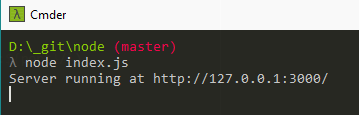
\includegraphics[width=0.90\textwidth]{img/consolejs.png}
	\end{center}
	\legend{Fonte: elaborado pela autora}
\end{figure}
% ---
% ----------------------------------------------------------
\section{Métodos e Etapas}\label{sec:metodos-etapas}
% ----------------------------------------------------------

A primeira fase deste trabalho se concentra no levantamento bibliográfico sobre \textit{Cloud Computing}, balanceamento de carga e Redes Neurais Artificiais. Nesta fase, o estudo se concentrou na pesquisa de serviços de \textit{Cloud} disponíveis no mercado, visto que o teste da ferramenta foi realizado a partir de uma infraestrutura hospedada em uma \textit{Cloud} real. 

A fase seguinte concentra-se na análise e levantamento das tecnologias utilizadas na implementação da estrutura para testes, inicialmente estudando tecnologias como a ferramenta CloudStack \cite{cloudstack} e a OpenStack \cite{openstack}. Devido à necessidade de possuir uma estrutura de servidores física, ambas as opções citadas foram descartadas e o serviço escolhido foi a EC2\cite{AmazonEC2}, fornecido pela AWS. Durante essa fase, ainda, houve o planejamento e estruturação do módulo que engloba a RNA, bem como sua arquitetura, posteriormente integrada ao módulo de balanceamento de carga. A arquitetura escolhida segue a estrutura descrita pela figura \ref{fig:arq}. 

\begin{figure}[htb]
	\caption{\label{fig:arq}Arquitetura simplificada do projeto}
	\begin{center}
		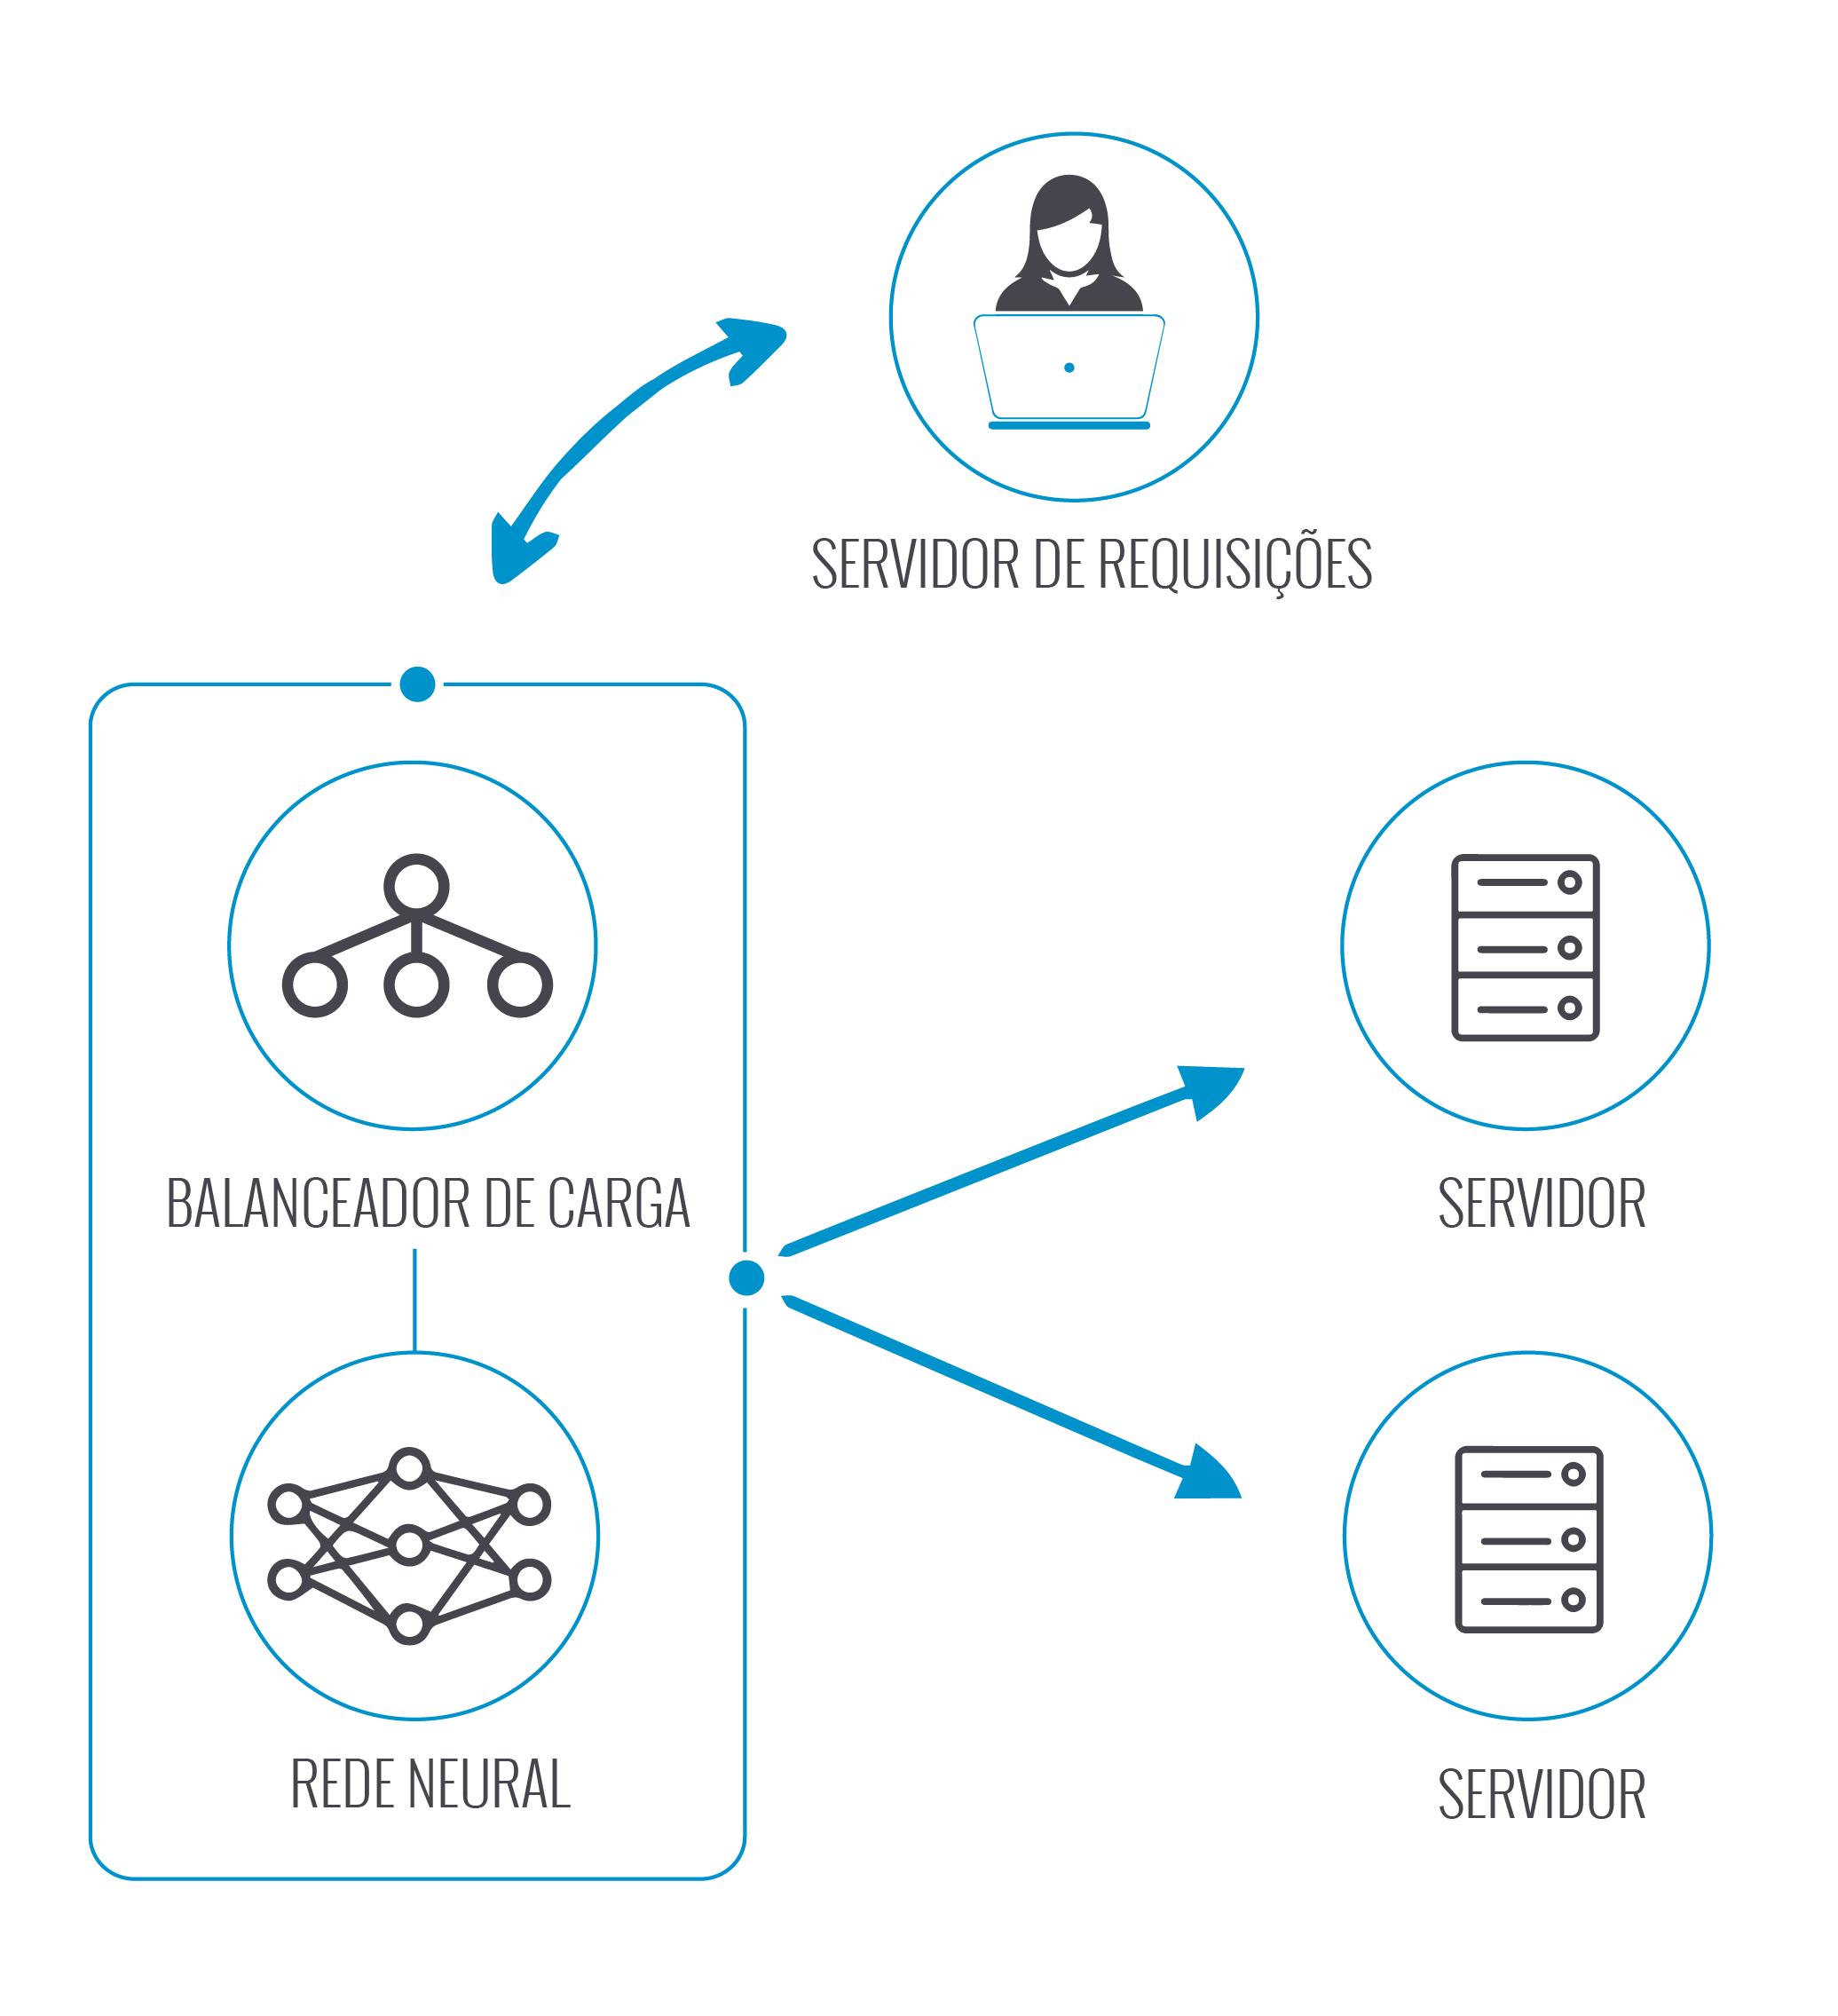
\includegraphics[width=0.50\textwidth]{img/projeto.png}
	\end{center}
	\legend{Fonte: elaborado pela autora}
\end{figure}

A arquitetura do projeto pode ser dividida em três módulos, como ilustrado na figura \ref{fig:arq}: o primeiro, consiste no servidor responsável pelo balanceamento de carga, o qual recebe todas as requisições que serão posteriormente direcionadas para o \textit{cluster} de servidores de dados; o segundo módulo é composto pelo \textit{cluster} de servidores de dados; e o terceiro é um servidor que gera requisições. Nesta arquitetura, a rede neural é um submódulo do balanceador, sendo responsável pela atribuição de pesos à cada um dos servidores presentes no \textit{cluster} de dados. Estes pesos são utilizados pelo algoritmo de balanceamento para direcionar as requisições aos servidores de modo equilibrado. 

A terceira fase do projeto concentrou-se na implementação e testes do módulo de balanceamento. Nessa fase, o estudo das tecnologias Nodejs e EC2 permitiu a implementação da aplicação e os testes com \textit{clusters} em nuvem.  Essa fase abrange, ainda, a análise do desempenho da abordagem escolhida, cujo resultado está descrito na seção de Resultados. A fase final do projeto se concentrou na escrita do relatório e apresentação dos resultados obtidos. 
 % inclui o arquivo metodologia.tex

% ----------------------------------------------------------


% ----------------------------------------------------------
% Desenvolvimento
% ----------------------------------------------------------
% ----------------------------------------------------------
% Metodologia
% ----------------------------------------------------------
\chapter{Arquitetura do projeto}\label{cap:desenvolvimento}
% ----------------------------------------------------------
% ----------------------------------------------------------

A arquitetura implementada para o módulo de balanceamento segue a proposta apresentada na figura \ref{fig:arq}. O processo de desenvolvimento foi dividido em módulos: \textit{Load Balancer} (balanceador de carga), \textit{Neural Network} (Rede Neural), \textit{Request Server} (servidor de requisições) e \textit{Servers}, sendo os dois primeiros parte integrante do protótipo de balanceamento de carga e os dois últimos utilizados para teste do protótipo. 

O \textbf{módulo de \textit{servers}} é composto por dois servidores do tipo t2.micro, conforme descrito na tabela \ref{tab:servidores}, cada um deles configurado como um servidor que recebe requisições em uma porta especifica e retorna o conteúdo solicitado. O objetivo do módulo do balanceador de carga é distribuir a carga de requisições entre estes servidores. Para executar e configurar estes servidores, fez-se uso do Nodejs, com código semelhante ao apresentado na seção \ref{sec:node-js}, cujo acesso está ilustrado na figura \ref{fig:serv-req}. 
\begin{figure}[htb]
	\caption{\label{fig:serv-req}Conexão ao servidor de Requisições}
	\begin{center}
		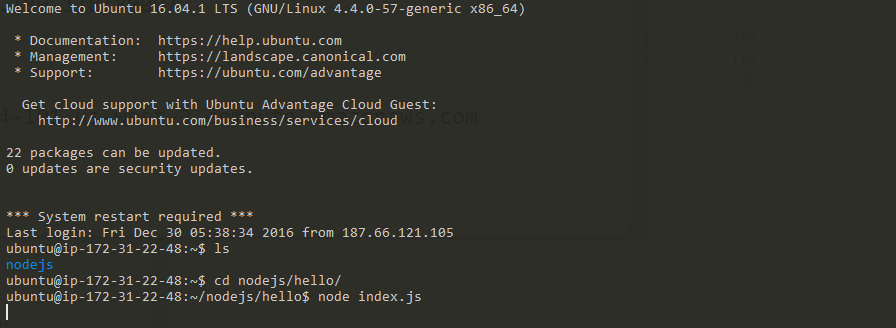
\includegraphics[width=0.90\textwidth]{img/servidor.png}
	\end{center}
	\legend{Fonte: elaborada pela autora}
\end{figure}

O \textbf{módulo de servidor de requisições} simula um cliente. Seu algoritmo gera aleatoriamente uma quantidade de solicitações ao servidor de balanceamento e aguarda a resposta da requisição, gravando em um arquivo de \textit{log} se a solicitação foi atendida com sucesso. 

O último módulo é o protótipo de aplicação em si, composto por duas partes: a primeira, é responsável pelo algoritmo de distribuição das requisições e a segunda implementa a Rede Neural Artificial. 

O \textbf{módulo de balanceamento de carga} recebe todas as requisições geradas pelo módulo de requisições e distribui entre os servidores. Para efetuar esta distribuição, escolheu-se utilizar o conceito do algoritmo de Round Robin \cite{nginx-rr}, no qual as requisições são distribuídas entre os servidores seguindo a ideia de turnos, ou seja, em uma lista de servidores, o balanceador de carga direciona a requisição para o primeiro, a próxima para o segundo da lista e assim por diante, até atingir o último servidor da lista, reiniciando o \textit{loop}. A figura \ref{fig:round} ilustra essa distribuição. 
\begin{figure}[htb]
	\caption{\label{fig:round}Round Robin}
	\begin{center}
		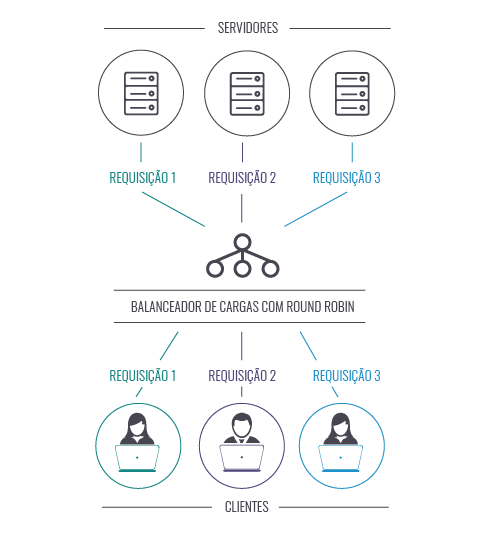
\includegraphics[width=0.70\textwidth]{img/rrobin-01.png}
	\end{center}
	\legend{Fonte: elaborada pela autora}
\end{figure}

\textit{Round Robin} é um algoritmo que tem como principal vantagem a estabilidade e a simplicidade de implementação e execução. Porém, sua eficiência ou precisão não é tão grande quando comparada à abordagens mais complexas pois muitos balanceadores não consideram as diferenças entre os servidores que recebem as requisições \cite{nginx-rr}. Por esta razão, há variantes de implementações de \textit{Round Robin} que buscam minimizar esta desvantagem, dentre elas o \textit{Round Robin} com pesos e \textit{Round Robin} dinâmico. O primeiro, atribui pesos aos servidores associados na lista e a distribuição é feita com base nesse atributo. Servidores com maior peso recebem mais requisições. A segunda variante associa os pesos dinamicamente, de acordo com a carga atual e a ociosidade de cada servidor. 

O módulo de balanceamento de carga, então, utiliza o conceito de Round Robin com pesos, atribuindo pesos aos servidores do módulo de \textit{servers}. Os pesos são definidos com base no \textbf{módulo de Rede Neural}, descrito a seguir. Ainda em relação ao módulo de balanceamento, a implementação do protótipo incorpora os pesos atribuídos, ou  melhor, a classificação advinda da Rede Neural Artificial para executar o balanceamento. Este módulo também é responsável por atualizar as informações das características dos servidores, utilizadas posteriormente na Rede Neural. 

Por fim, o \textbf{Módulo de Rede Neural} implementa a rede responsável por atribuir os pesos aos servidores presentes na lista de servidores. As características consideradas no processamento dos pesos estão descritas na tabela \ref{tab:caracteristicas}. A saída deste módulo é ligada diretamente ao módulo de balanceamento, através de um vetor que indica quais servidores estão aptos a receber requisições. 

% ---
\section{Arquitetura da Rede Neural}\label{sec:ann}
% ---

A seção \ref{sec:rna} apresenta alguns modelos de arquiteturas que podem ser aplicadas para resolver problemas de classificação. Como discutido nesta mesma seção, a arquitetura do tipo de RNA ou abordagem utilizada para resolver um problema que envolva aprendizado está diretamente relacionada ao tipo de problema que se deseja resolver com determinada técnica. Este trabalho tem definido em seus objetivos aplicar uma Rede Neural Artificial para aprender se os servidores gerenciados pelo \textbf{módulo de balanceamento} estão aptos a realizar uma requisição. 

Como discutido na seção \ref{sec:balanceamento-carga}, este tipo de aplicação deve considerar elementos como distribuição esparsa da arquitetura em núvem, capacidade de armazenamento, complexidade do algoritmo e pontos de falhas, tempo de resposta, utilização de recursos, dentre outros critérios que determinam a eficiência de uma aplicação de balanceamento. 

Diante do problema, este trabalho considerou que, ao incorporar ao algoritmo de balanceamento uma RNA, um critério crucial para a escolha de sua arquitetura está diretamente ligada às características citadas anteriormente. Portanto, elementos como tempo de resposta e complexidade do algoritmo receberam certa prioridade em relação ao desempenho da rede na classificação em si. Como discutido na seção \ref{sec:rna}, a escolha da arquitetura, suas funções de ativação, tipo de aprendizado, e, principalmente, número de camadas e neurônios, são características que impactam diretamente no tempo de processamento. Redes com muitas camadas, como as CNNs, por exemplo, levam um tempo consideravelmente alto no aprendizado e possuem uma arquitetura sofisticada. 

Considerando que a RNA escolhida seria incorporada ao \textbf{módulo de balanceamento} e que, por ser uma aplicação de balanceamento de carga de requisições - onde o tempo de resposta é importantíssimo - o modelo escolhido foi o Perceptron, por ser de simples implementação. Além disso, a definição das características também permitiu que este modelo se apresentasse como uma boa escolha, visto que o número de características é pequeno e o problema de classificação, neste caso, não exige uma função tão complexa de separação dos dados no espaço de características. 

Portanto, este trabalho considerou como critério de escolha da rede a simplicidade da implementação da RNA para diminuir a complexidade do \textbf{módulo de balanceamento}, dimensão do problema (em relação às suas características) e tempo de resposta. Tendo isto em vista, o modelo escolhido foi o Perceptron e a arquitetura da rede está descrita a seguir. 

% ---
\textbf{Definição de características}

A tabela \ref{tab:caracteristicas} descreve as características que a RNA recebe como \textit{input}. Cada uma delas impacta diretamente no desempenho da distribuição das requisições. O tipo de servidor, apesar de ser um parâmetro estático (ou seja, não muda ao longo da execução), quando colocado em conjunto com as demais características, torna-se importante. Por exemplo, um servidor que possui maior capacidade de processamento e está à uma distância maior do que um servidor com menor capacidade e mais próximo pode ter um tempo de resposta semelhante, equilibrando o peso do servidor em relação aos demais. 

\begin{table}[h]
	\caption{Características}
	\centering
	\small
	\renewcommand{\arraystretch}{1.2} % Aumenta espaçamento vertical
	\begin{tabular}{>{\centering\arraybackslash}m{3.5cm} m{11.5cm}}
		\hline 
		\textbf{Característica} & \textbf{Descrição}  \\ 
		\hline 
		\textbf{Tipo de servidor}& t2.micro ou t2.medium - servidores com maior poder de processamento podem receber um número maior de requisições \\ 
		\hline 
		\textbf{Tempo de resposta } & Tempo para receber e responder à requisição\\ 
		\hline 
		\textbf{Estado} & Indica se o servidor está apto à receber requisições\\ 
		\hline 
		\textbf{Distâcia} & Atribui um valor de distância (física) para o servidor - Neste caso, servidores mais distantes demoram mais para responder\\ 
		\hline 
	\end{tabular}\\
	\vspace{3mm}
	\legend{Elaborado pela autora.}
	\label{tab:caracteristicas}
\end{table}

Características como tempo de resposta e estado são dinâmicas, ou seja, mudam ao longo da execução do algoritmo. Essas características impactam diretamente na decisão, visto que, um servidor que recebe muitas requisições (ou seja, está sobrecarregado) em uma iteração pode, na seguinte, estar livre, caso consiga responder à todas as requisições em sua fila. 
A discussão acerca da escolha destas características e sua efetividade é apresentada no capítulo de \ref{cap:resultados}.

% ---
\textbf{Implementação da Rede Neural com Perceptron}


A Rede Neural escolhida segue a ideia de Perceptron apresentada na seção \ref{sec:rna}. A rede contem três camadas: uma de entrada, uma escondida e uma camada de saída. Por se tratar de uma rede neural aplicada à balanceamento de carga, alguns conceitos foram levados em conta ao estabelecer a forma de aprendizado dinâmico.Pelas razões elencadas no início desta seção, a rede neural escolhida possui poucas camadas, como ilustrado pela figura \ref{fig:rede}, com o objetivo de aumentar a velocidade de processamento e garantir que o tempo de resposta do balanceador não seja tão afetado pelo tempo de processamento da RNA. Além disto, a quantidade de características e o tipo de saída esperada na arquitetura proposta por este projeto permitem uma implementação de uma rede deste tipo. 

\begin{figure}[htb]
	\caption{\label{fig:rede} Camadas implementadas na rede neural}
	\begin{center}
		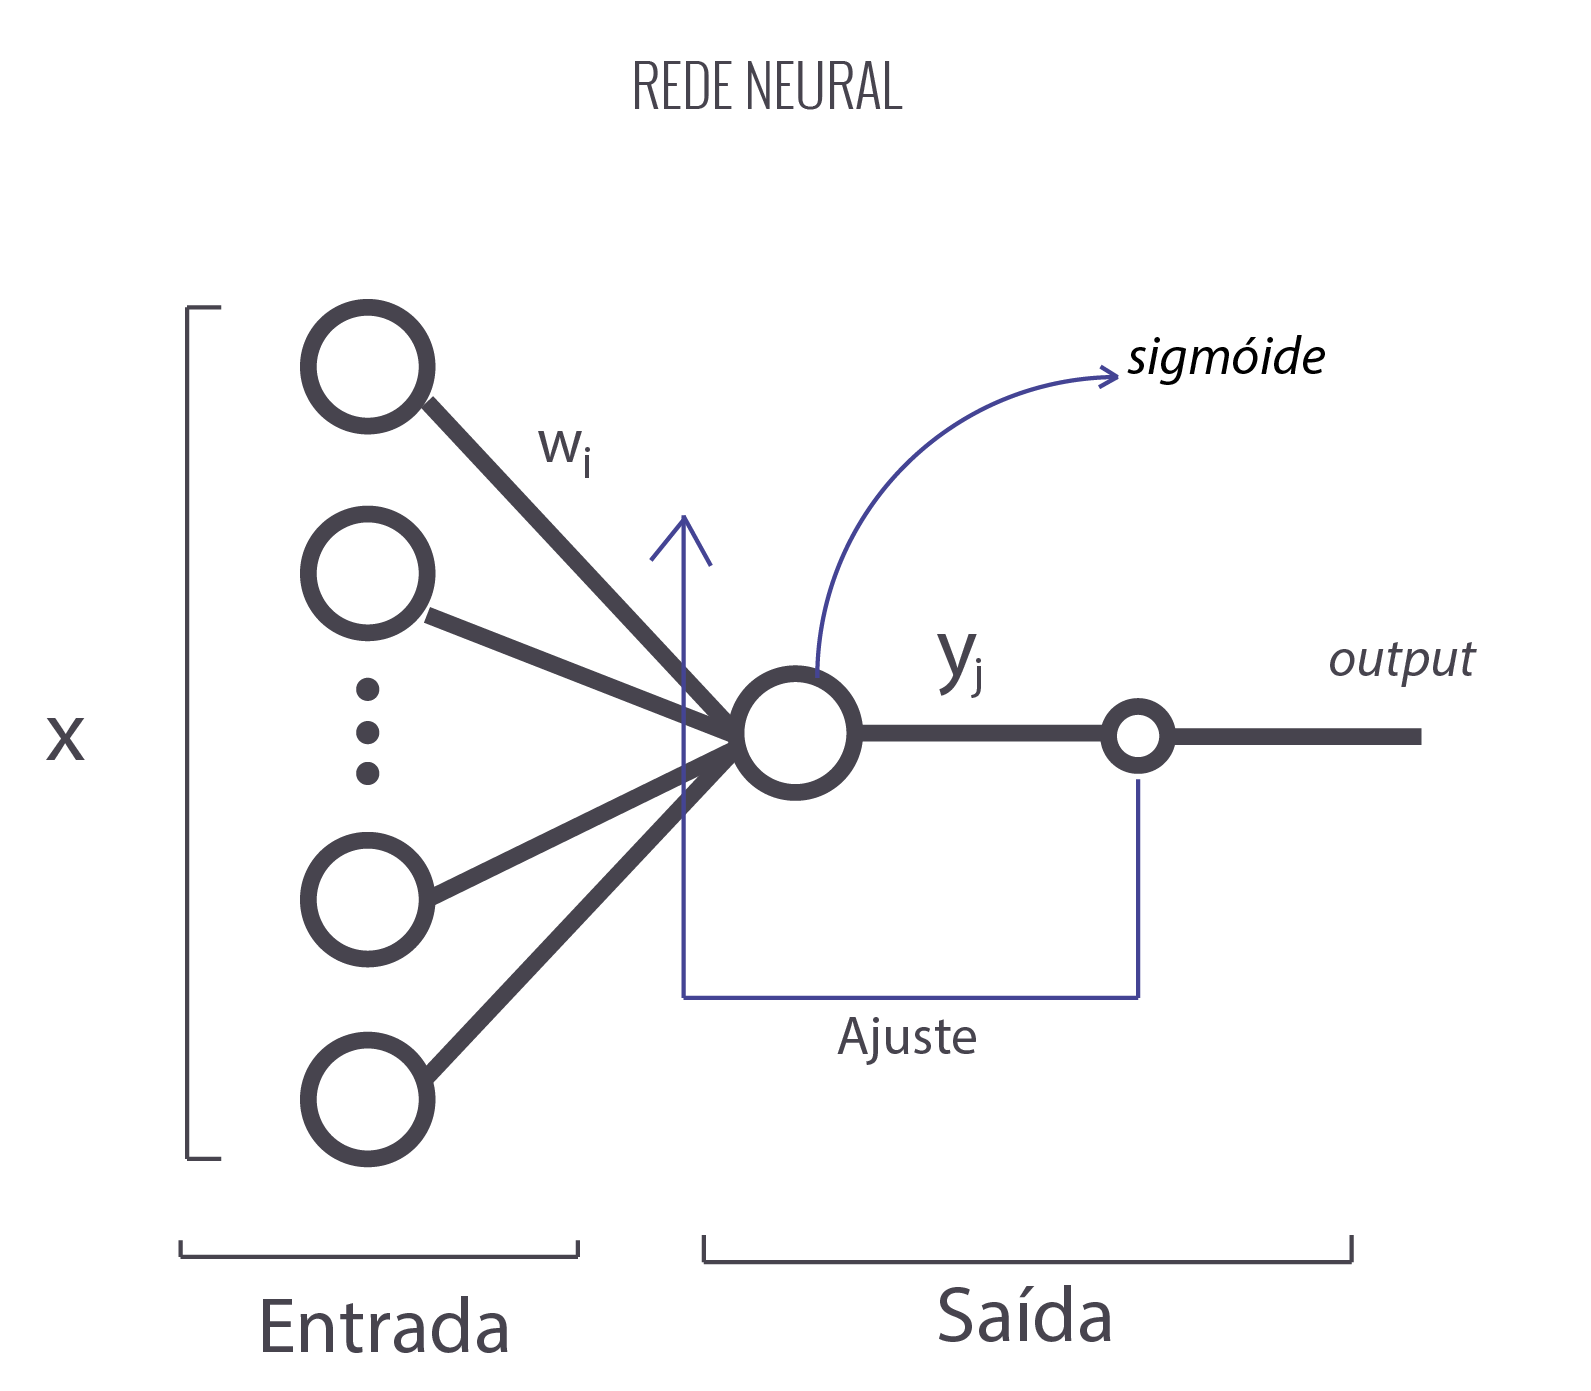
\includegraphics[width=0.60\textwidth]{img/redeusada.png}
	\end{center}
	\legend{Fonte: elaborada pela autora}
\end{figure}

A primeira camada presente na arquitetura da rede neural é a camada de entrada. É composta por um vetor $x$ de tamanho $n$, sendo $n$ igual ao número de características (apresentadas na tabela \ref{tab:caracteristicas}) do servidor. Os pesos que essas características tem na classificação são armazenados em $w$. Em teoria, $w$ consiste em uma matriz que possui $n$ linhas (quantidade de \textit{inputs}) e $m$ colunas (quantidade de \textit{outputs}). Como a saída é a classificação se o servidor está apto à receber a requisição, ou seja, o \textit{output} da rede é a classificação como "apto" ou "não apto", um único neurônio nesta camada é suficiente, logo, neste caso, $w$ passa a ser um vetor de pesos. 

As sinapses ou propagação de sinal da primeira camada para a segunda é feita seguindo o cálculo na equação \ref{eq:pesos}. 
\begin{equation}
x_i = x_i \times w_i
\label{eq:pesos}
\end{equation}

A segunda camada realiza um somatório das características (\ref{eq:sum}) e aplica a função sigmoide da equação \ref{eq:sigmoide} ao resultado. $y_j$ é a variável que guarda o valor do somatório da iteração $j$. Antes de aplicar a sigmoide, os valores são multiplicados por 0.02 para diminuir a faixa de valores na saída. 

\begin{equation}
y_j = \sum_{i=1}^{n} {x_i}
\label{eq:sum}
\end{equation}


\begin{equation}
S(y_j) =  \frac{1}{(1 + e ^ {y_j} )} 
\label{eq:sigmoide}
\end{equation}

A última camada utiliza o \textit{output} para ajustar os pesos em $w$. Esta é a fase de treinamento da rede, que ocorre de maneira dinâmica. Ao fim da classificação, o \textit{output} identifica o servidor como "apto" ou "não apto" a receber requisições. Se for classificado como "apto", e a requisição for direcionada para ele então a classificação foi correta o algoritmo ajusta o peso que mais influenciou a decisão, seguindo a equação \ref{eq:weight}. Caso a classificação seja incorreta, e a requisição retornou uma falha ou o servidor não conseguiu atender a requisição, o ajuste de peso diminui o peso da característica que mais influenciou a decisão, seguindo a equação \ref{eq:weight2}

\begin{equation}
w_i = w_i + 0.5
\label{eq:weight}
\end{equation}

\begin{equation}
w_i = w_i - 0.5
\label{eq:weight2}
\end{equation}

Ao fim do processamento, os valores de $w$ são salvos para uso posterior. A ideia de manter o treinamento constante da rede advém de sua implementação mais simples, que permite velocidade no processamento e atribuição dos valores de pesos utilizados pelo balanceador de cargas, visto que os as entradas mudam de maneira rápida e o treinamento depende dos resultados anteriores. 

% ---
\section{Implementação e Testes}\label{sec:testes}
% ---

Por se tratar de uma aplicação de \textit{backend} implementada em Nodejs, o protótipo não possui interface gráfica, de modo que sua interface de comandos é feita pelo terminal, como pode ser observado na Figura \ref{fig:consoleann}. Ao iniciar o acesso, o balanceador verifica quais servidores estão ativos e os coloca em uma lista, como apresentado na Figura \ref{fig:areas}. Então, a aplicação verifica a conexão com cada um dos servidores na lista, para garantir que o mesmo possui o estado saudável. 

Em seguida, são atribuídas os valores das características para cada servidor na lista, seguindo a definição apresentada na tabela \ref{tab:caracteristicas}. Caso seja a primeira vez que a aplicação de balanceamento é executada, $w$ é preenchido com valores padrões. Caso contrário, dados salvos em um arquivo que guarda as informações de peso do processamento anterior são carregados. 


A implementação foi feita em Nodejs e o código está disponível no Github\footnote{\url{https://github.com/ksetoue}} da autora. O algoritmo implementado para balanceamento de cargas com a rede neural segue os seguintes passos: 
\begin{enumerate}
	\item \textit{inicialização de paramêtros}: inicialização do vetor de pesos, objeto que armazena dados dos servidores;
	\item \textit{se nova requisição recebida}: 
	\begin{enumerate}
		\item classificar cada servidor (chamar a RNA)
		\item escolher a melhor opção para direcionar a requisição 
		\item verifica se a requisição foi atendida 
		\item manda o resultado para o cliente 			
	\end{enumerate}
	\item \textit{Ajustar os pesos}: conforme descrito em \ref{sec:ann};
	\item \textit{Caso desativado}: salvar paramêtros de peso; 
	\item \textit{Senão}: voltar ao primeiro item; 
\end{enumerate}

As figuras \ref{fig:consoleann}, \ref{fig:areas} e \ref{fig:weights} apresentam a interface no console da aplicação de balanceamento em execução. As informações apresentadas são a lista de servidores ativos e os pesos mais recentes. 

\begin{figure}[htb]
	\caption{\label{fig:consoleann} \textit{Screenshot} de teste realizado com a Rede Neural}
	\begin{center}
		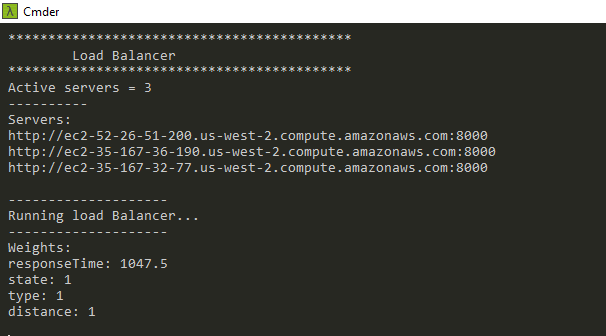
\includegraphics[width=0.70\textwidth]{img/load-bal-app.png}
	\end{center}
	\legend{Fonte: elaborada pela autora}
\end{figure}

Esta parte da aplicação corresponde ao \textbf{módulo de balanceamento}, executado no servidor t2.medium. 

\begin{figure}[htb]
	\caption{\label{fig:areas} \textit{Screenshot} Dados do Balanceador - Servidores Ativos}
	\begin{center}
		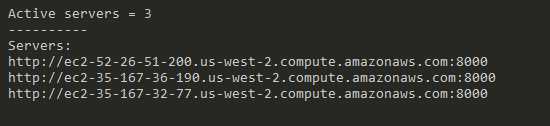
\includegraphics[width=0.80\textwidth]{img/activeservers.png}
	\end{center}
	\legend{Fonte: elaborada pela autora}
\end{figure}

\begin{figure}[htb]
	\caption{\label{fig:weights} \textit{Screenshot} Dados do Balanceador - Pesos mais recentes (RNA)}
	\begin{center}
		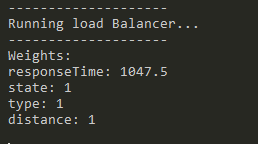
\includegraphics[width=0.50\textwidth]{img/weights.png}
	\end{center}
	\legend{Fonte: elaborada pela autora}
\end{figure}





 % inclui o arquivo desenvolvimento.tex

% ----------------------------------------------------------
% Resultados
% ----------------------------------------------------------
% ----------------------------------------------------------
% Desenvolvimento
% ----------------------------------------------------------
\chapter{Resultados}\label{cap:resultados}
% ----------------------------------------------------------

Os experimentos realizados para verificar o desempenho do balanceador foram realizados em ambiente real, de maneira dinâmica através da execução dos três módulos da aplicação. Foram alocados três servidores do tipo t2.micro como servidores, um servidor t2.medium para alocar a aplicação de balanceamento e um computador para executar a aplicação para executar as requisições, no qual é armazenado o log das requisições. 
\begin{figure}[htb]
	\caption{\label{fig:tests} \textit{Screenshot} Aplicação para testar o balanceador}
	\begin{center}
		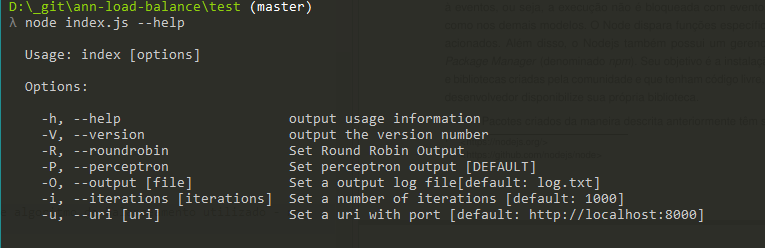
\includegraphics[width=0.70\textwidth]{img/testeapp.png}
	\end{center}
	\legend{Fonte: elaborada pela autora}
\end{figure}
Definiu-se um total de 100 requisições para avaliar o desempenho do balanceador com a Rede Neural. Para realizar os testes foi implementado uma aplicação na qual seleciona-se o tipo de algoritmo de balanceamento utilizado - no caso, a RNA ou Round Robin puro - número de iterações e url onde está hospedado o servidor de balanceamento (Figura \ref{fig:tests}). Esta aplicação armazena um arquivo de log com as informações de todas as requisições enviadas e as respostas (incluindo o servidor que atendeu a requisição). 

A avaliação do desempenho da aplicação de balanceamento foi comparada ao balanceamento realizado com Round Robin puro, através da análise dos arquivos de log gerados em ambos os casos de teste, com o mesmo número de requisições com o qual foi testada a aplicação de RNA. É fato que a aplicação de balanceamento teve desempenho satisfatório, visto que conseguiu distribuir a carga das requisições entre os servidores com sucesso, sem apresentar uma diferença significativa em relação ao algoritmo de Round Robin puro. 

Durante o processo foi possível notar que a característica que mais influenciou o processo de escolha foi a quantidade de requisições associadas ao servidor. Percebe-se também que servidores do mesmo tipo tendem a deixar o balanceamento mais equilibrado. 

A tabela \ref{tab:results} apresenta a quantidade de requisições atribuídas a cada um dos $k$ servidores alocados após executar 100 iterações na aplicação que gera requisições. Nos testes, os $k=3$ servidores são tipo t2.micro. A comparação é feita entre o balanceamento realizado com Round Robin, com a RNA sem treinamento e com a RNA após o aprendizado dos pesos.  

\begin{table}[ht]
	\caption{Comparação entre Distribuição de requisições entre servidores}
	\centering
	\begin{tabular}{c c c c}
		\hline 
		Servidores & Round Robin & RNA & RNA - treinada\\ 
		\hline 
		Servidor 1 & 34 & 36 & 37 \\ 
		\hline 
		Servidor 2 & 35 & 35 & 37 \\ 
		\hline 
		Servidor 3 & 34 & 36 & 32 \\ 
		\hline 
	\end{tabular} \\
	\vspace{3mm}
	\legend{Elaborado pela autora.}
	\label{tab:results}
\end{table}

É possível notar que não há diferença significativa entre os dois algoritmos, em relação à atribuir requisições de forma desigual. Na última coluna da tabela, nota-se que o Servidor 3 recebeu um número menor de requisições, em relação aos demais. Isto pode ter ocorrido devido à oscilações na rede. As Figuras \ref{fig:resultann}, \ref{fig:resultann2} e \ref{fig:resultrr} apresentam \textit{screenshots} dos testes. 

\begin{figure}[htb]
	\caption{\label{fig:resultann} \textit{Screenshot} Teste com RNA}
	\begin{center}
		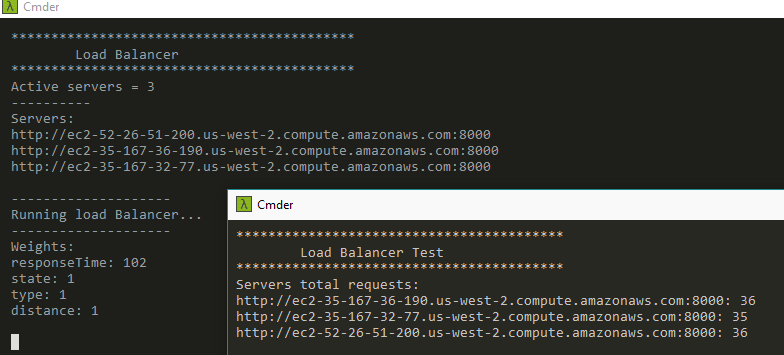
\includegraphics[width=0.70\textwidth]{img/resquisicao-ann.png}
	\end{center}
	\legend{Fonte: elaborada pela autora}
\end{figure}
\begin{figure}[htb]
	\caption{\label{fig:resultann2} \textit{Screenshot} Teste com RNA já treinada}
	\begin{center}
		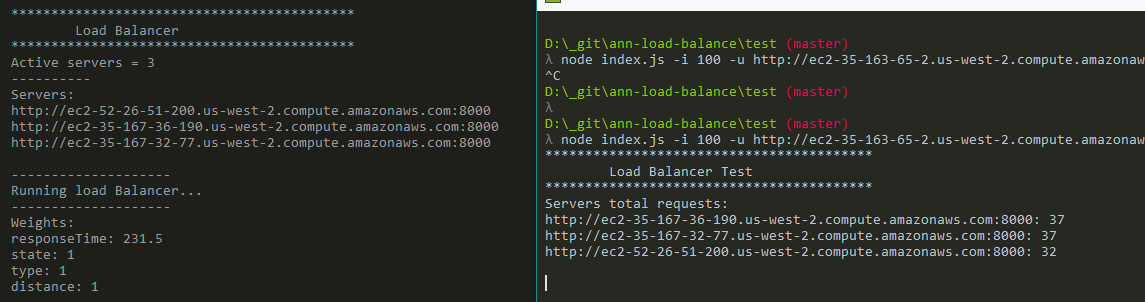
\includegraphics[width=0.90\textwidth]{img/resquisicao-ann-second.png}
	\end{center}
	\legend{Fonte: elaborada pela autora}
\end{figure}

\vspace{-10cm}

\begin{figure}[htb]
	\caption{\label{fig:resultrr} \textit{Screenshot} Teste com Round Robin}
	\begin{center}
		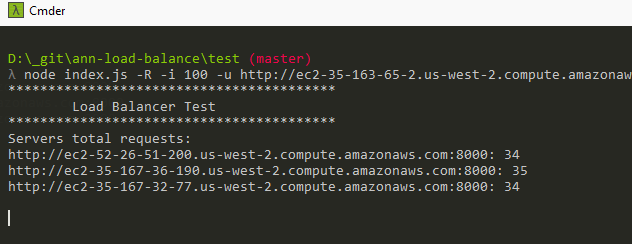
\includegraphics[width=0.70\textwidth]{img/resquisicao-round.png}
	\end{center}
	\legend{Fonte: elaborada pela autora}
\end{figure}
% ----------------------------------------------------------
 % inclui o arquivo resultados.tex

% ----------------------------------------------------------


% ----------------------------------------------------------
% Conclusão
% ----------------------------------------------------------
\chapter{Conclusão}
% ----------------------------------------------------------
O presente trabalho apresenta uma aplicação de balanceamento de cargas utilizando Redes Neurais Artificiais como Perceptron, como um módulo funcional de balanceamento de requisições. Seu desempenho foi analisado através da comparação com um algoritmo conhecido e bastante usado, o Round Robin. 

Os testes demonstram ganho significativo no uso da RNA. Portanto, nas condições em que os testes foram realizados, podemos considerar o Round Robin como melhor alternativa, se levarmos em conta a simplicidade de sua implementação.  
No entanto, visto que o modelo proposto neste trabalho leva em consideração os estados mais recentes dos servidores, levando em conta seu último estado, esta implementação tende a apresentar melhor desempenho, visto que a distribuição das cargas se dá pela avaliação de estados como falhas de conexão e estado do servidor, por exemplo.


% ---
\subsection{Trabalhos futuros}\label{sec:futuro}
% ---
Como sugestão de trabalhos futuros pode-se considerar analisar o desempenho da arquitetura desta aplicação de balanceamento em ambientes instáveis, com servidores distintos. Além disto, propor outras características e avaliar o desempenho com base nesta escolha. Em relação à rede, testar e avaliar o desempenho da aplicação com outras arquiteturas de Redes Neurais Artificiais, com mais camadas, por exemplo. 
% ----------------------------------------------------------

% ----------------------------------------------------------------------------------------------------------------------------------



% ----------------------------------------------------------
% ELEMENTOS PÓS-TEXTUAIS
% ----------------------------------------------------------

% ----------------------------------------------------------
% Referências bibliográficas
% ----------------------------------------------------------
\bibliography{referencias}
% ----------------------------------------------------------


\end{document}
